%=============================================================================
%  Medieval Field Cannon -- OpenGL project report
%  Build:  pdflatex report.tex   (run twice for the table of contents)
%=============================================================================
\documentclass[11pt,a4paper]{article}

\usepackage[a4paper,margin=24mm,headheight=14pt]{geometry}
\usepackage[T1]{fontenc}
\usepackage{lmodern}
\usepackage{amsmath,amssymb,bm}
\usepackage{graphicx}
\usepackage{booktabs}
\usepackage{xcolor}
\usepackage{microtype}
\usepackage{caption}
\usepackage{subcaption}
\usepackage{float}
\usepackage{fancyhdr}
\usepackage{listings}
\usepackage{enumitem}
\usepackage{tikz}
\usetikzlibrary{positioning,arrows.meta,calc,fit,backgrounds,decorations.pathreplacing}
\usepackage[hidelinks]{hyperref}

\graphicspath{{images/}}

\definecolor{accent}{RGB}{140,72,20}
\definecolor{codebg}{RGB}{247,247,244}
\definecolor{codekw}{RGB}{20,90,150}
\definecolor{codecm}{RGB}{110,120,110}

\lstdefinestyle{code}{
  backgroundcolor=\color{codebg},
  basicstyle=\ttfamily\scriptsize,
  keywordstyle=\color{codekw}\bfseries,
  commentstyle=\color{codecm}\itshape,
  stringstyle=\color{accent},
  numbers=none, frame=single, rulecolor=\color{black!20},
  breaklines=true, showstringspaces=false,
  columns=fullflexible, xleftmargin=6pt, framexleftmargin=6pt,
  aboveskip=8pt, belowskip=8pt,
}
\lstset{style=code}
\lstdefinelanguage{GLSL}{
  keywords={void,vec2,vec3,vec4,mat3,mat4,float,bool,int,if,else,return,uniform,varying,
            in,out,attribute,const,discard},
  morekeywords=[2]{normalize,length,max,min,clamp,pow,dot,reflect,mix,exp,ftransform},
  keywordstyle=\color{codekw}\bfseries,
  keywordstyle=[2]\color{accent},
  comment=[l]{//}, morecomment=[s]{/*}{*/},
  sensitive=true,
}

\pagestyle{fancy}
\fancyhf{}
\fancyhead[L]{\small Medieval Field Cannon --- OpenGL}
\fancyhead[R]{\small\thepage}
\renewcommand{\headrulewidth}{0.3pt}

\newcommand{\bs}{\bm{s}}
\newcommand{\bN}{\bm{N}}
\newcommand{\bL}{\bm{L}}
\newcommand{\bV}{\bm{V}}
\newcommand{\bR}{\bm{R}}
\newcommand{\bH}{\bm{H}}
\newcommand{\bP}{\bm{P}}
\newcommand{\bM}{\bm{M}}
\newcommand{\bT}{\bm{T}}
\newcommand{\key}[1]{\textsf{\small\textbf{#1}}}

\title{\vspace{-14mm}\textbf{A Medieval Field Cannon in OpenGL}\\[2mm]
       \large Hierarchical Transformations, Rolling Constraints and the
       Phong Reflection Model}
\author{Computer Graphics Project Report}
\date{\today}

\begin{document}
\maketitle
\thispagestyle{fancy}

\begin{abstract}
\noindent
This report documents a real-time 3-D scene, written in Python with PyOpenGL and
freeglut, of a medieval field cannon on a wheeled carriage.  The carriage can be
driven along the ground with the wheels rolling at exactly the right rate, the
barrel elevates about its trunnions, recoils along its own axis as a damped
spring when fired, and launches a cannonball that follows a ballistic arc.  The
whole assembly is built from analytic primitives whose surface normals are
derived rather than approximated, and is lit by a single movable point light
using the full Phong reflection model --- evaluated \emph{per fragment} in GLSL,
with a per-vertex fixed-function path available for direct comparison.  Every
quantitative claim in this document is reproduced by \texttt{verify.py}, whose
output is included verbatim in Appendix~\ref{app:verify}, and every figure is a
real frame captured from the running program.
\end{abstract}

\vspace{-4mm}
\tableofcontents
\vspace{4mm}

%=============================================================================
\section{Introduction}
%=============================================================================

The brief was to build a scene that \emph{visibly} demonstrates a small set of
core computer-graphics ideas rather than to build a large one.  The cannon is a
good vehicle for this because each required concept maps onto a physical part of
the object:

\begin{itemize}[itemsep=2pt,topsep=3pt]
  \item the carriage \textbf{translates}, and its wheels must \textbf{rotate} at
        the rate implied by that translation, or the illusion collapses
        instantly;
  \item the barrel \textbf{rotates about a pivot that is itself carried by the
        moving carriage}, which is exactly what a hierarchical transformation
        is for;
  \item the barrel \textbf{translates along its own rotated axis} when it
        recoils, which cannot be expressed in world coordinates without first
        composing the parent transforms;
  \item the wooden carriage and the iron barrel react to light in obviously
        different ways, which is the clearest possible evidence that a real
        lighting model is running rather than flat colours.
\end{itemize}

\begin{figure}[H]
  \centering
  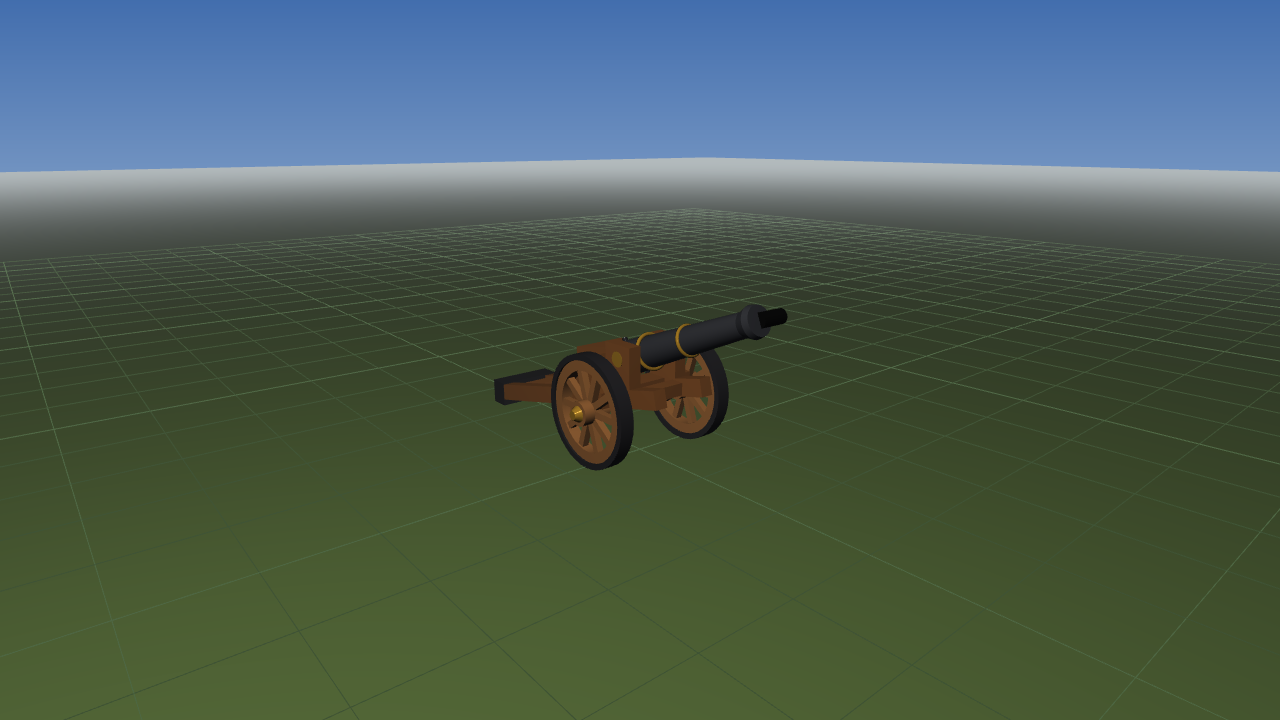
\includegraphics[width=\linewidth]{01_overview}
  \caption{The complete scene.  Oak carriage, iron-tyred spoked wheels, brass
  fittings and a cast-iron barrel, lit by one orbiting point light over a
  1\,m reference grid.  Per-fragment Phong shading; exponential-squared fog
  dissolves the far edge of the ground plane into the sky.}
  \label{fig:overview}
\end{figure}

\subsection{Requirement coverage}

\begin{table}[H]
\centering\small
\begin{tabular}{@{}p{58mm}p{60mm}p{30mm}@{}}
\toprule
\textbf{Requirement} & \textbf{Where it is implemented} & \textbf{Evidence} \\
\midrule
Translation & \texttt{Cannon.drive}, root \texttt{glTranslatef} & Fig.~\ref{fig:roll} \\
Rotation (rolling) & $\varphi=-s/R$ in \texttt{Cannon.drive} & Fig.~\ref{fig:roll}, \S\ref{sec:roll} \\
Rotation (elevation) & \texttt{glRotatef} at the trunnion pivot & Fig.~\ref{fig:elev} \\
Hierarchical / composite transforms & \texttt{Cannon.draw} push/pop tree & \S\ref{sec:hier}, Fig.~\ref{fig:tree} \\
Perspective projection + camera & \texttt{gluPerspective}, \texttt{gluLookAt} & \S\ref{sec:view}, Fig.~\ref{fig:cams} \\
Phong lighting (ambient, diffuse, specular) & \texttt{lighting.py} + GLSL & \S\ref{sec:phong}, Fig.~\ref{fig:lightoff} \\
Two contrasting materials & matte oak vs.\ shiny cast iron & Fig.~\ref{fig:materials} \\
Continuous animation / interactivity & recoil spring, projectile, light orbit & Fig.~\ref{fig:recoil},~\ref{fig:arc} \\
\bottomrule
\end{tabular}
\caption{Mapping from the assessment criteria to the implementation.}
\end{table}

%=============================================================================
\section{How to run the project}
%=============================================================================

\subsection{Prerequisites}

\begin{table}[H]
\centering\small
\begin{tabular}{@{}lll@{}}
\toprule
\textbf{Component} & \textbf{Requirement} & \textbf{Version used for this report} \\
\midrule
Python      & 3.9 or newer            & 3.14.5 (64-bit, Windows 11) \\
PyOpenGL    & $\ge$ 3.1.7             & 3.1.10 \\
NumPy       & $\ge$ 1.24              & 2.4.4 \\
Pillow      & $\ge$ 10.0 (screenshots only) & 12.2.0 \\
GPU / driver& OpenGL 2.0+ compatibility profile & AMD Radeon 760M, GL 4.6 compat.\ (GLSL 4.60) \\
\bottomrule
\end{tabular}
\end{table}

\noindent
On Windows the PyOpenGL wheel ships \texttt{freeglut64.vc14.dll} inside
\texttt{OpenGL/DLLS/}, so \textbf{no separate freeglut download is needed}.  On
Linux install \texttt{freeglut3-dev} (Debian/Ubuntu:
\texttt{sudo apt install freeglut3-dev}); on macOS GLUT ships with the system
but is deprecated, and the compatibility profile is capped at OpenGL 2.1 ---
the program still runs, falling back where necessary.

\subsection{Installation}

\begin{lstlisting}[language=bash]
cd Graphics-project
python -m pip install -r requirements.txt      # PyOpenGL, numpy, Pillow
python test.py                                 # sanity check: a coloured triangle
\end{lstlisting}

\noindent
If \texttt{test.py} shows a red/green/blue triangle, the toolchain is ready.

\subsection{Running}

\begin{lstlisting}[language=bash]
python main.py                     # interactive scene
python verify.py                   # numerical self-checks (no window needed)
python main.py --shots docs/images # re-render every figure in this report, then exit
\end{lstlisting}

\subsection{Controls}
\label{sec:controls}

\begin{table}[H]
\centering\small
\begin{tabular}{@{}llll@{}}
\toprule
\textbf{Key} & \textbf{Action} & \textbf{Key} & \textbf{Action} \\
\midrule
\key{$\leftarrow$} / \key{$\rightarrow$} & drive backward / forward (wheels roll) & \key{L} & light on / off \\
\key{$\uparrow$} / \key{$\downarrow$}    & elevate / depress the barrel ($0^\circ$--$45^\circ$) & \key{K} & light orbit on / off \\
\key{Space} & fire: flash, recoil, cannonball & \key{N} & point light $\leftrightarrow$ directional \\
\key{C} & cycle the five camera presets & \key{[} \key{]} & nudge the light azimuth \\
mouse drag & orbit the camera & \key{F} & per-fragment Phong $\leftrightarrow$ per-vertex Gouraud \\
wheel, \key{+} / \key{-} & zoom & \key{B} & Phong $\leftrightarrow$ Blinn--Phong specular \\
\key{W} & wireframe & \key{M} & cycle the barrel material \\
\key{G} & ground plane on / off & \key{T} & projectile trails on / off \\
\key{J} & reference grid on / off & \key{X} & clear the projectiles \\
\key{H} & help overlay & \key{U} & HUD on / off \\
\key{R} & reset everything & \key{P} & save a PNG screenshot \\
\key{Esc} / \key{Q} & quit & & \\
\bottomrule
\end{tabular}
\caption{Complete key bindings.  The arrow keys are level-triggered: hold them.}
\end{table}

\subsection{Files}

\begin{table}[H]
\centering\small
\begin{tabular}{@{}lp{108mm}@{}}
\toprule
\textbf{File} & \textbf{Responsibility} \\
\midrule
\texttt{main.py}       & Window and GL setup, camera, input handling, HUD, main loop, and the
                         \texttt{--shots} driver that renders the report figures. \\
\texttt{cannon.py}     & The \texttt{Cannon} class: dimensions, animation state, the transformation
                         hierarchy, and the numpy mirror of that hierarchy used to locate the muzzle. \\
\texttt{lighting.py}   & \texttt{Material} definitions, the \texttt{Light} rig, the GLSL Phong program,
                         the fog setup and the \texttt{unlit} context manager. \\
\texttt{projectile.py} & Cannonball integration, ground bounce, fading trail, and the closed-form
                         range predictor used by the HUD. \\
\texttt{utils.py}      & Analytic primitive meshes (box, frustum, tube, sphere, torus, ground) with
                         derived normals, a display-list cache, and 2-D text helpers. \\
\texttt{verify.py}     & Numerical checks of every formula quoted in this report. \\
\texttt{test.py}       & Toolchain sanity check (single triangle). \\
\bottomrule
\end{tabular}
\end{table}

\subsection{Troubleshooting}

\begin{table}[H]
\centering\small
\begin{tabular}{@{}p{54mm}p{92mm}@{}}
\toprule
\textbf{Symptom} & \textbf{Cause and fix} \\
\midrule
\texttt{ModuleNotFoundError: OpenGL} & PyOpenGL is not installed for \emph{this} interpreter.  Run
   \texttt{python -m pip install PyOpenGL}. \\
\texttt{OpenGL.error.NullFunctionError:\newline glutInit} & freeglut cannot be loaded.  On Linux install
   \texttt{freeglut3-dev}; on Windows reinstall PyOpenGL so the bundled DLL is present. \\
Console prints \emph{``GLSL unavailable''} & The driver rejected the shader.  The program
   automatically uses the fixed-function per-vertex path; everything still works, and
   \key{F} simply has no effect. \\
The window opens but stays black & A remote/software GL context without a depth buffer.  Try
   forcing the vendor GPU, or run with the integrated GPU driver updated. \\
\texttt{--shots} writes black PNGs & Some drivers refuse to read an occluded back buffer.  Keep the
   window visible and unobstructed while it runs (it takes about two seconds). \\
\bottomrule
\end{tabular}
\end{table}

%=============================================================================
\section{Architecture}
%=============================================================================

The program is a classic single-threaded GLUT application.  \texttt{glutIdleFunc}
advances the simulation by the measured wall-clock $\Delta t$ (clamped to
$50$\,ms so a stalled frame cannot teleport the cannon) and requests a redraw;
\texttt{glutDisplayFunc} renders.  One frame is:

\begin{enumerate}[itemsep=1pt,topsep=3pt]
  \item clear, then paint the three-stop sky gradient in an orthographic pass
        with depth writes disabled;
  \item load the projection ($\texttt{gluPerspective}$) and view
        ($\texttt{gluLookAt}$) matrices;
  \item upload the light position --- \emph{after} the view matrix, because
        OpenGL stores \texttt{GL\_POSITION} pre-multiplied by the modelview
        matrix current at the moment of the call, i.e.\ in eye space;
  \item bind the Phong shader (or fall back to fixed-function lighting);
  \item draw the ground, the cannon hierarchy, the projectiles, and the light
        marker;
  \item draw the HUD in a second orthographic pass with lighting and fog off.
\end{enumerate}

Every primitive mesh is generated once and compiled into a display list
(\texttt{utils.\_cached}), so the per-frame CPU cost is a handful of
\texttt{glCallList} calls rather than thousands of Python-level
\texttt{glVertex3f} calls.

%=============================================================================
\section{The mathematics}
%=============================================================================

\subsection{Homogeneous coordinates and affine transforms}

Points are written $\tilde{\bP}=(x,y,z,1)^{\mathsf T}$ and directions
$(x,y,z,0)^{\mathsf T}$.  The trailing $0$ is not cosmetic: it makes a direction
immune to translation, which is why \texttt{Cannon.muzzle\_state} can obtain the
barrel's axis by pushing $(1,0,0,0)^{\mathsf T}$ through the very same matrix
that positions the muzzle tip.  The two transforms this project needs are

\begin{equation}
\bT(t_x,t_y,t_z)=
\begin{pmatrix}1&0&0&t_x\\0&1&0&t_y\\0&0&1&t_z\\0&0&0&1\end{pmatrix},
\qquad
\bm{R}_z(\theta)=
\begin{pmatrix}
\cos\theta&-\sin\theta&0&0\\
\sin\theta&\phantom{-}\cos\theta&0&0\\
0&0&1&0\\0&0&0&1
\end{pmatrix}.
\label{eq:tr}
\end{equation}

Both the elevation of the barrel and the spin of the wheels are rotations about
$+Z$, because the scene is laid out with $+X$ forward, $+Y$ up and $+Z$ to the
right, so $Z$ is the axle direction and also the axis the barrel swings in.

\subsection{The matrix stack is a scene-graph traversal}
\label{sec:hier}

OpenGL's modelview stack turns a tree into code.  \texttt{glTranslatef} and
\texttt{glRotatef} \emph{post}-multiply the current matrix,
$\bM \leftarrow \bM\bm{A}$, and \texttt{glPushMatrix}/\texttt{glPopMatrix}
save and restore it.  A depth-first walk of the tree, pushing on the way down
and popping on the way back up, therefore leaves every node with the product of
all the transforms on its path from the root --- which is precisely the
definition of a hierarchical transformation.  Reading the code from top to
bottom is reading the matrix product from left to right.

\begin{figure}[H]
\centering
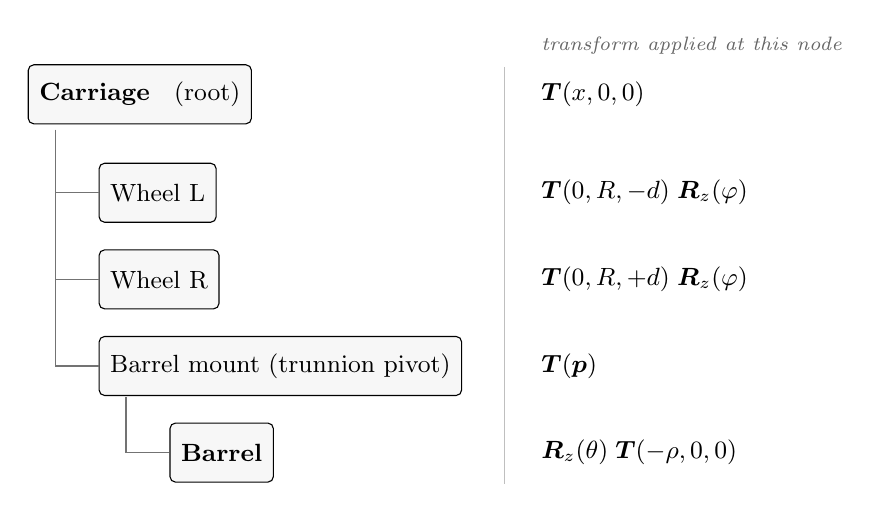
\begin{tikzpicture}[
  every node/.style={font=\small},
  box/.style={draw,rounded corners=2pt,anchor=west,inner sep=4pt,
              fill=black!3,minimum height=7.5mm},
  op/.style={font=\small,anchor=west},
  lab/.style={font=\scriptsize\itshape,anchor=west,text=black!60},
  edge/.style={draw=black!55,line width=0.5pt}
]
\def\ta{6.4}                                  % x of the transform column
\node[box] (root)   at (0.0,  0.0) {\textbf{Carriage} \; (root)};
\node[box] (wl)     at (0.9, -1.25) {Wheel L};
\node[box] (wr)     at (0.9, -2.35) {Wheel R};
\node[box] (mount)  at (0.9, -3.45) {Barrel mount (trunnion pivot)};
\node[box] (barrel) at (1.8, -4.55) {\textbf{Barrel}};

\foreach \n/\y in {wl/-1.25, wr/-2.35, mount/-3.45}{
  \draw[edge] (0.35,-0.45) |- (0.9,\y);
}
\draw[edge] (1.25,-3.85) |- (1.8,-4.55);

\node[op] at (\ta,  0.00) {$\bT(x,0,0)$};
\node[op] at (\ta, -1.25) {$\bT(0,R,-d)\;\bm{R}_z(\varphi)$};
\node[op] at (\ta, -2.35) {$\bT(0,R,+d)\;\bm{R}_z(\varphi)$};
\node[op] at (\ta, -3.45) {$\bT(\bm{p})$};
\node[op] at (\ta, -4.55) {$\bm{R}_z(\theta)\;\bT(-\rho,0,0)$};

\node[lab] at (\ta,  0.62) {transform applied at this node};
\draw[black!25,line width=0.4pt] (\ta-0.35,0.35) -- (\ta-0.35,-4.95);
\end{tikzpicture}
\caption{The scene graph.  $x$ is the carriage position, $\varphi$ the wheel
angle, $\bm{p}$ the trunnion pivot, $\theta$ the elevation and $\rho$ the recoil
offset.  Depth $=2$: shallow on purpose.}
\label{fig:tree}
\end{figure}

Writing $\bm{V}$ for the view matrix, the composite matrices are

\begin{align}
\bM_{\text{carriage}} &= \bm{V}\,\bT(x,0,0), \label{eq:mc}\\
\bM_{\text{wheel}}    &= \bM_{\text{carriage}}\,\bT(0,R,\pm d)\,\bm{R}_z(\varphi),\\
\bM_{\text{mount}}    &= \bM_{\text{carriage}}\,\bT(\bm{p}),\\
\bM_{\text{barrel}}   &= \bM_{\text{mount}}\,\bm{R}_z(\theta)\,\bT(-\rho,0,0).
\label{eq:mb}
\end{align}

The essential observation is that $\bM_{\text{barrel}}$ contains
$\bT(x,0,0)$: driving the carriage moves the barrel, the trunnions, the wheels
and the muzzle together, for free, because they are all descendants.  Check~6 of
\texttt{verify.py} confirms this numerically --- changing only $x$ from
$0$ to $4$\,m displaces the muzzle by exactly $(4,0,0)$\,m while the elevation
is held at $25^\circ$.

\subsection{Rolling without slipping}
\label{sec:roll}

\begin{figure}[H]
\centering
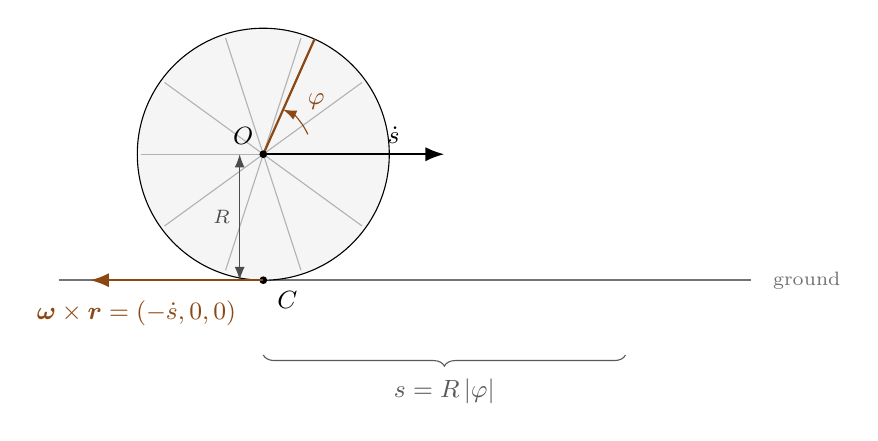
\begin{tikzpicture}[scale=1.0,every node/.style={font=\small}]
  \draw[line width=0.6pt,black!55] (-2.6,-1.6) -- (6.2,-1.6);
  \node[black!55,font=\scriptsize,anchor=west] at (6.35,-1.6) {ground};
  \draw[fill=black!4] (0,0) circle (1.6);
  \foreach \a in {0,36,...,324} \draw[black!30] (0,0) -- (\a:1.55);
  \draw[thick,accent] (0,0) -- (66:1.6);
  \draw[accent,->,>=Latex] (24:0.62) arc (24:66:0.62);
  \node[accent,font=\small] at (45:0.95) {$\varphi$};
  \fill (0,0) circle (1.4pt); \node[anchor=south east,inner sep=2pt] at (-0.05,0.04) {$O$};
  \draw[<->,>=Latex,black!70] (-0.30,0) -- node[anchor=east,font=\scriptsize,pos=0.5]{$R$} (-0.30,-1.6);
  \fill (0,-1.6) circle (1.4pt);
  \node[anchor=north west,inner sep=2pt] at (0.10,-1.66) {$C$};
  \draw[-{Latex[length=2.4mm]},thick] (0,0) -- node[anchor=south,pos=0.72]{$\dot{s}$} (2.3,0);
  \draw[-{Latex[length=2.4mm]},thick,accent] (0,-1.6) -- (-2.2,-1.6);
  \node[accent,anchor=north east,font=\small] at (-0.22,-1.74)
       {$\bm{\omega}\times\bm{r}=(-\dot{s},0,0)$};
  \draw[decorate,decoration={brace,amplitude=4pt,mirror},black!65]
       (0,-2.55) -- node[anchor=north,pos=0.5,yshift=-5pt]{$s = R\,|\varphi|$} (4.6,-2.55);
\end{tikzpicture}
\caption{The rolling constraint.  The material point at the contact $C$ must be
instantaneously at rest, so the spin exactly cancels the translation.}
\label{fig:rollmath}
\end{figure}

For a wheel of radius $R$ whose centre translates with velocity
$\dot{\bs}=(\dot{s},0,0)$ and which spins with angular velocity
$\bm{\omega}=(0,0,\omega_z)$, the velocity of the material point at the ground
contact, whose position relative to the centre is $\bm{r}=(0,-R,0)$, is

\begin{equation}
\bm{v}_C=\dot{\bs}+\bm{\omega}\times\bm{r}
        =(\dot{s},0,0)+(0,0,\omega_z)\times(0,-R,0)
        =(\dot{s}+\omega_z R,\;0,\;0).
\end{equation}

Rolling without slipping means $\bm{v}_C=\bm{0}$, hence
$\omega_z=-\dot{s}/R$, and integrating from rest,

\begin{equation}
\boxed{\;\varphi=-\frac{s}{R}\;}
\qquad\text{(radians; the code stores degrees, }
\varphi^\circ=-\tfrac{180}{\pi}\tfrac{s}{R}\text{).}
\label{eq:roll}
\end{equation}

The minus sign is not decoration: with $+Z$ pointing right, a wheel advancing
towards $+X$ turns \emph{clockwise} as seen from $+Z$, which is a negative
rotation under the right-hand rule.  Get it wrong and the wheels visibly spin
backwards, the single most recognisable animation bug there is.

Implementation (\texttt{cannon.py}) applies \eqref{eq:roll} incrementally, using
the distance actually moved after clamping so that pushing against the end of
the field does not accumulate phantom rotation:

\begin{lstlisting}[language=Python]
new_x  = clamp(self.x + ds, X_MIN, X_MAX)
moved  = new_x - self.x
self.x = new_x
self.wheel_angle -= math.degrees(moved / WHEEL_RADIUS)
\end{lstlisting}

\noindent
\textbf{Check.}  Driving $s=2.6000$\,m with $R=0.6200$\,m gives
$\varphi=-240.2726^\circ$ analytically and $-240.2726^\circ$ in the simulation
(error $2.7\times10^{-12}$ degrees, i.e.\ floating-point round-off); the rim arc
$R|\varphi|$ recovers $2.6000$\,m.  Figure~\ref{fig:roll} is that exact
manoeuvre.

\begin{figure}[H]
  \centering
  \begin{subfigure}{0.49\linewidth}
    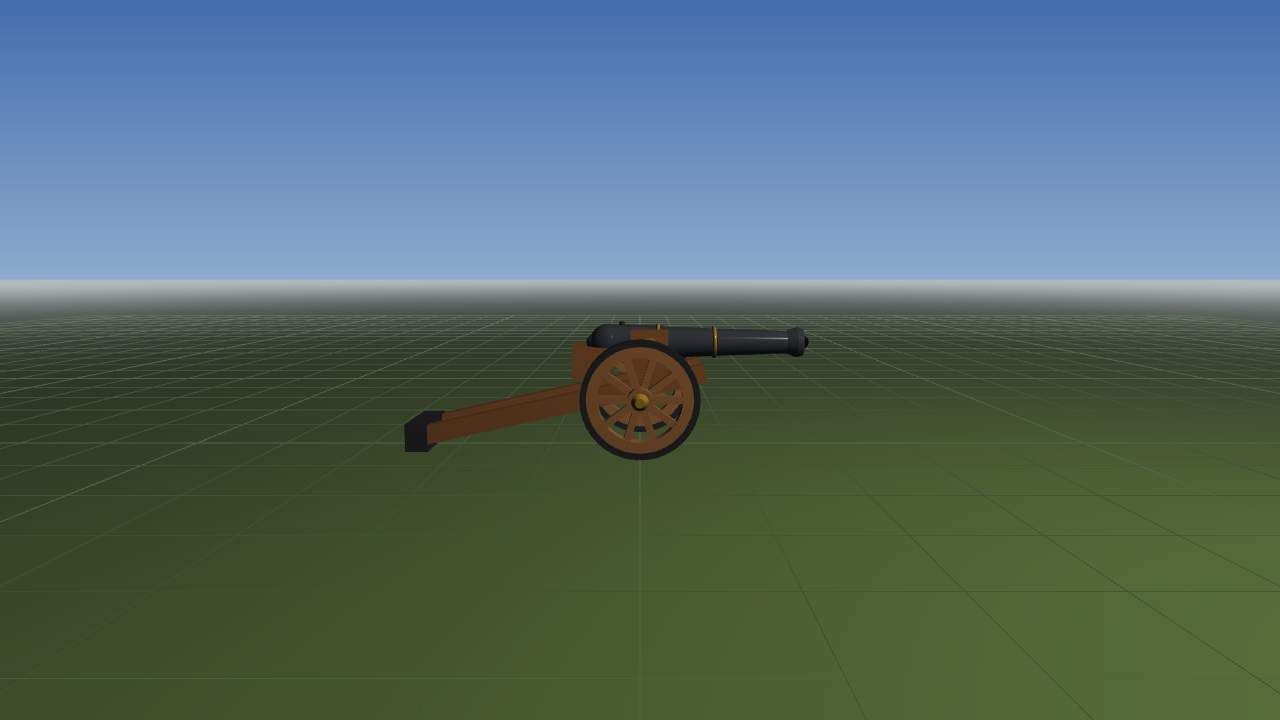
\includegraphics[width=\linewidth]{03_roll_before}
    \caption{$s=0$, $\varphi=0^\circ$}
  \end{subfigure}\hfill
  \begin{subfigure}{0.49\linewidth}
    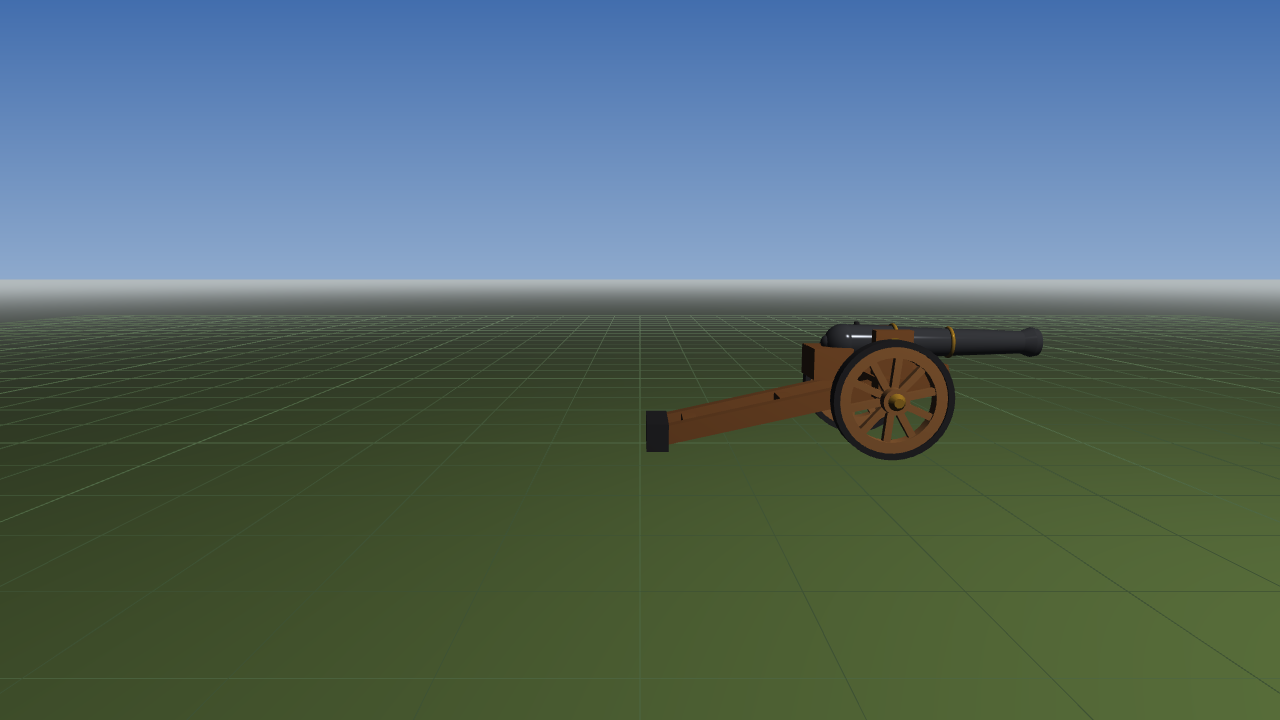
\includegraphics[width=\linewidth]{04_roll_after}
    \caption{$s=2.60$\,m, $\varphi=-240.27^\circ$}
  \end{subfigure}
  \caption{Translation and the rolling constraint, from a camera fixed in
  \emph{world} space so both effects are visible at once.  The carriage has
  advanced 2.6 grid squares and the spokes have turned through
  $-240.27^\circ$ --- two thirds of a turn, which is why the spoke pattern
  (10 spokes, $36^\circ$ apart) does not repeat.}
  \label{fig:roll}
\end{figure}

\subsection{Rotation about a pivot that is not the origin}

A rotation matrix rotates about the origin.  To rotate about an arbitrary point
$\bm{p}$ one conjugates:

\begin{equation}
\bm{R}_{\bm{p}}(\theta)=\bT(\bm{p})\,\bm{R}_z(\theta)\,\bT(-\bm{p}).
\label{eq:pivot}
\end{equation}

In the renderer the $\bT(-\bm{p})$ factor is absent, and this is deliberate
rather than an omission: the barrel mesh is \emph{authored} in a local frame
whose origin already sits at the trunnion, so the geometry arrives
pre-multiplied by $\bT(-\bm{p})$ in the modelling stage.  What the code writes,

\begin{lstlisting}[language=Python]
glTranslatef(*PIVOT)                      # T(p)
glRotatef(self.elevation, 0, 0, 1)        # Rz(theta)
self._draw_trunnions()                    # stays with the mount
glTranslatef(-self.recoil, 0, 0)          # T(-rho) along the barrel's own axis
self._draw_barrel()
\end{lstlisting}

\noindent
is \eqref{eq:pivot} with the inverse translation folded into the model.  Note
where the trunnions are drawn: after the elevation rotation but \emph{before}
the recoil translation, so they swing with the barrel but do not slide with it,
exactly as the real hardware behaves.

\begin{figure}[H]
  \centering
  \begin{subfigure}{0.32\linewidth}
    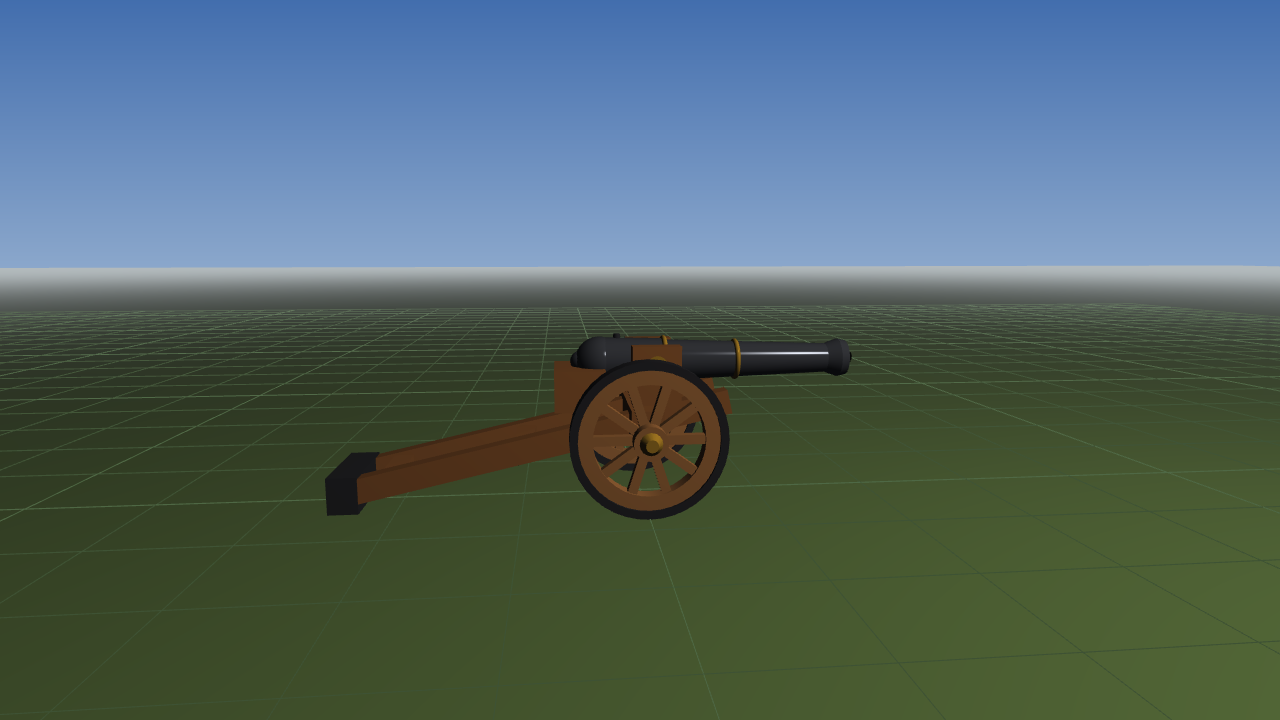
\includegraphics[width=\linewidth]{05_elev_00}\caption{$\theta=0^\circ$}
  \end{subfigure}\hfill
  \begin{subfigure}{0.32\linewidth}
    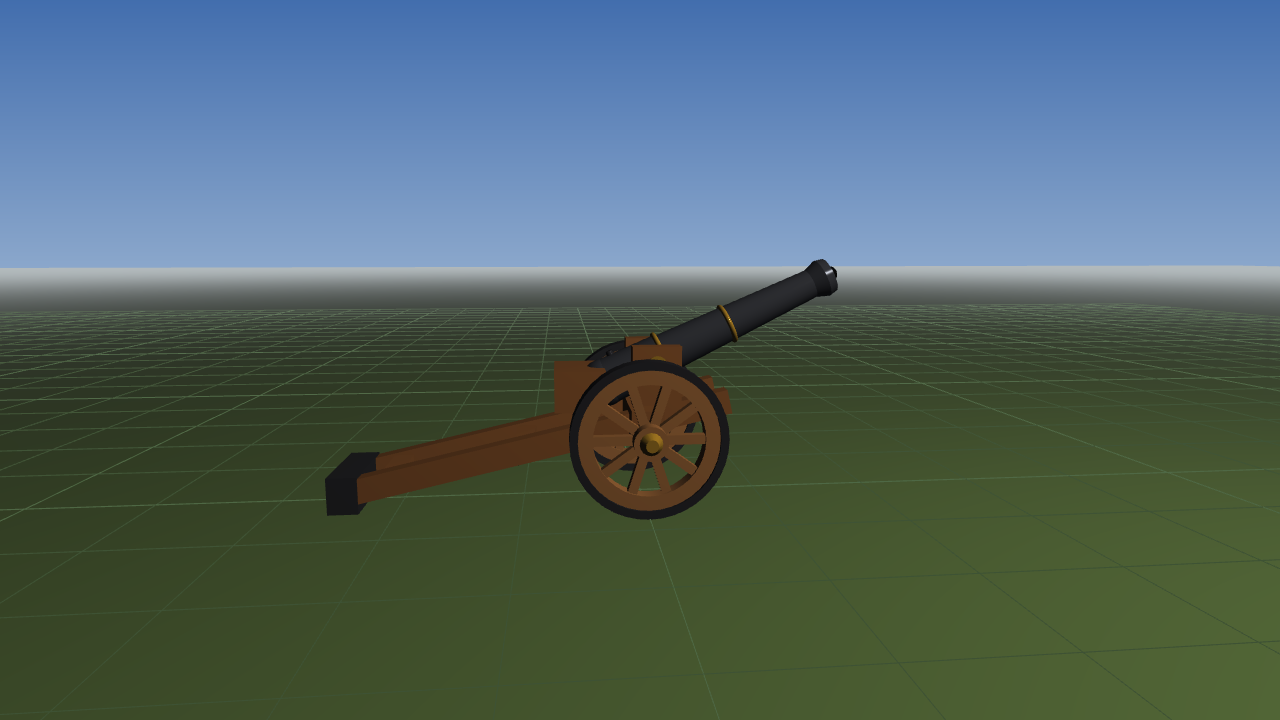
\includegraphics[width=\linewidth]{06_elev_25}\caption{$\theta=25^\circ$}
  \end{subfigure}\hfill
  \begin{subfigure}{0.32\linewidth}
    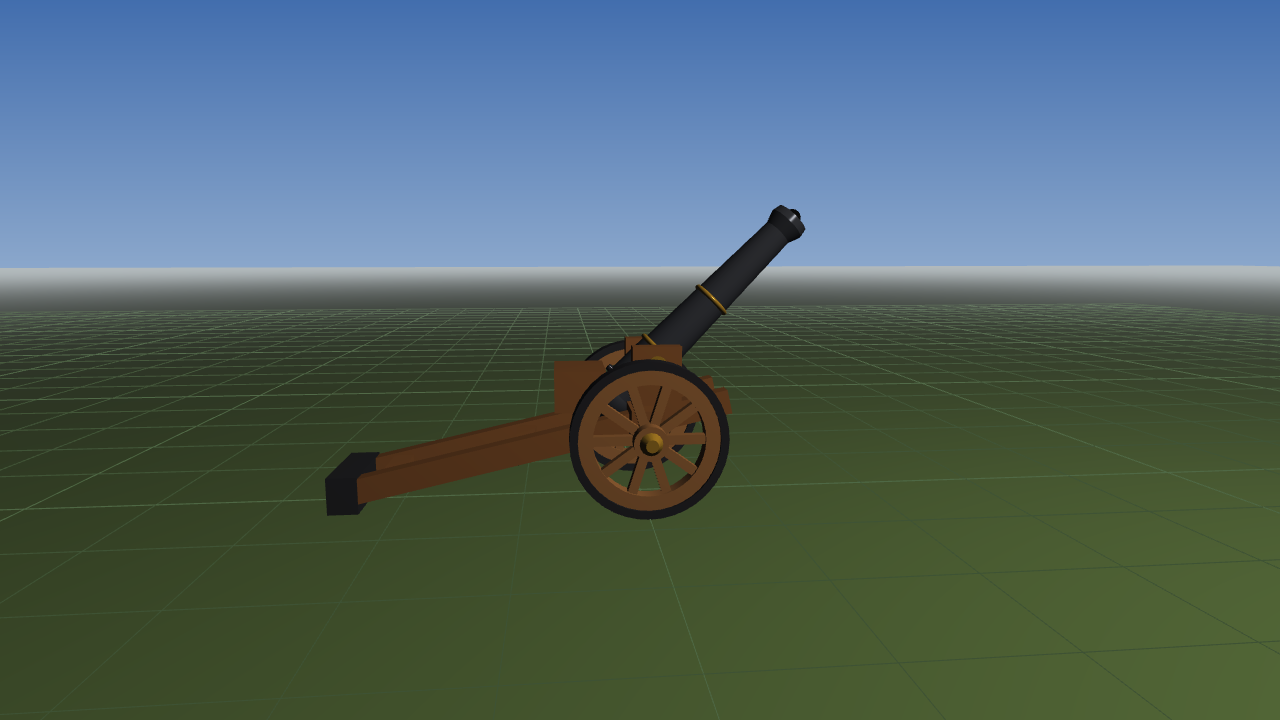
\includegraphics[width=\linewidth]{07_elev_45}\caption{$\theta=45^\circ$}
  \end{subfigure}
  \caption{Elevation, clamped to $[0^\circ,45^\circ]$.  The pivot stays fixed in
  the carriage while the muzzle sweeps an arc of radius
  $\ell=1.70$\,m about it; the camera and light are identical in all three
  frames.}
  \label{fig:elev}
\end{figure}

\subsection{Where is the muzzle?}

Firing needs the world position and direction of the muzzle, and guessing them
with trigonometry written a second time is how the ball ends up leaving from
inside the barrel.  Instead \texttt{Cannon.barrel\_matrix} rebuilds
\eqref{eq:mb} in numpy --- the same factors in the same order --- and pushes two
vectors through it:

\begin{equation}
\tilde{\bm{q}}=\bM_{\text{barrel}}^{\text{(world)}}\begin{pmatrix}\ell\\0\\0\\1\end{pmatrix},
\qquad
\tilde{\bm{d}}=\bM_{\text{barrel}}^{\text{(world)}}\begin{pmatrix}1\\0\\0\\0\end{pmatrix},
\qquad \ell = 1.70\,\text{m}.
\end{equation}

Expanding the product gives the closed form

\begin{equation}
\bm{q}=\bigl(x+p_x+(\ell-\rho)\cos\theta,\;\;p_y+(\ell-\rho)\sin\theta,\;\;0\bigr),
\qquad
\bm{d}=(\cos\theta,\sin\theta,0),
\label{eq:muzzle}
\end{equation}

and \texttt{verify.py} confirms the matrix chain and \eqref{eq:muzzle} agree to
$0.000\times10^{0}$\,m at $\theta\in\{0^\circ,32^\circ,45^\circ\}$ with
$\rho\in\{0,0.30\}$\,m.  Because $\tilde{\bm{d}}$ carries $w=0$ it picks up the
rotation but not the translations, so it is already the unit barrel axis
($|\bm{d}|=1.000000$).

\subsection{Recoil as a damped harmonic oscillator}

On firing, the barrel is given a backwards impulse and then pulled home by an
elastic mount.  Writing $\rho(t)\ge 0$ for the distance the barrel has slid back
along its own axis,

\begin{equation}
\ddot{\rho}+c\,\dot{\rho}+k\,\rho=0,
\qquad \rho(0)=0,\quad \dot{\rho}(0)=v_0 ,
\label{eq:ode}
\end{equation}

with $k=90.0\;\mathrm{s^{-2}}$, $c=2\zeta\sqrt{k}=16.128\;\mathrm{s^{-1}}$ and
$v_0=3.40\;\mathrm{m/s}$.  The natural frequency, damping ratio and damped
frequency are

\begin{equation}
\omega_n=\sqrt{k}=9.4868\ \mathrm{rad/s},\qquad
\zeta=\frac{c}{2\sqrt{k}}=0.850,\qquad
\omega_d=\omega_n\sqrt{1-\zeta^2}=4.9975\ \mathrm{rad/s},
\end{equation}

so the system is \emph{under}-damped ($\zeta<1$) --- chosen deliberately, since a
critically damped return ($\zeta=1$) creeps back and reads as sluggish, whereas
a small overshoot looks mechanical.  The solution of \eqref{eq:ode} is

\begin{equation}
\rho(t)=\frac{v_0}{\omega_d}\,e^{-\zeta\omega_n t}\sin(\omega_d t),
\qquad
t_{\max}=\frac{1}{\omega_d}\arctan\!\frac{\omega_d}{\zeta\omega_n},
\label{eq:recoilsol}
\end{equation}

giving $t_{\max}=0.1110$\,s and $\rho_{\max}=0.1464$\,m.  The renderer does not
evaluate \eqref{eq:recoilsol}; it integrates \eqref{eq:ode} with semi-implicit
(symplectic) Euler,

\begin{equation}
\dot{\rho}\leftarrow\dot{\rho}+\bigl(-k\rho-c\dot{\rho}\bigr)\Delta t,
\qquad
\rho\leftarrow\rho+\dot{\rho}\,\Delta t ,
\end{equation}

which stays stable at interactive time-steps.  Measured against
\eqref{eq:recoilsol}:

\begin{table}[H]
\centering\small
\begin{tabular}{@{}rrrr@{}}
\toprule
$\Delta t$ & peak $\rho$ (m) & $t$ of peak (s) & error vs.\ \eqref{eq:recoilsol} \\
\midrule
$1/240$  & 0.1375 & 0.108 & 6.09\,\% \\
$1/480$  & 0.1419 & 0.110 & 3.05\,\% \\
$1/4000$ & 0.1459 & 0.111 & 0.37\,\% \\
\bottomrule
\end{tabular}
\caption{First-order convergence of the recoil integrator; the barrel settles to
within 2\,\% of rest after $\approx 0.55$\,s in every case.}
\end{table}

\begin{figure}[H]
  \centering
  \begin{subfigure}{0.49\linewidth}
    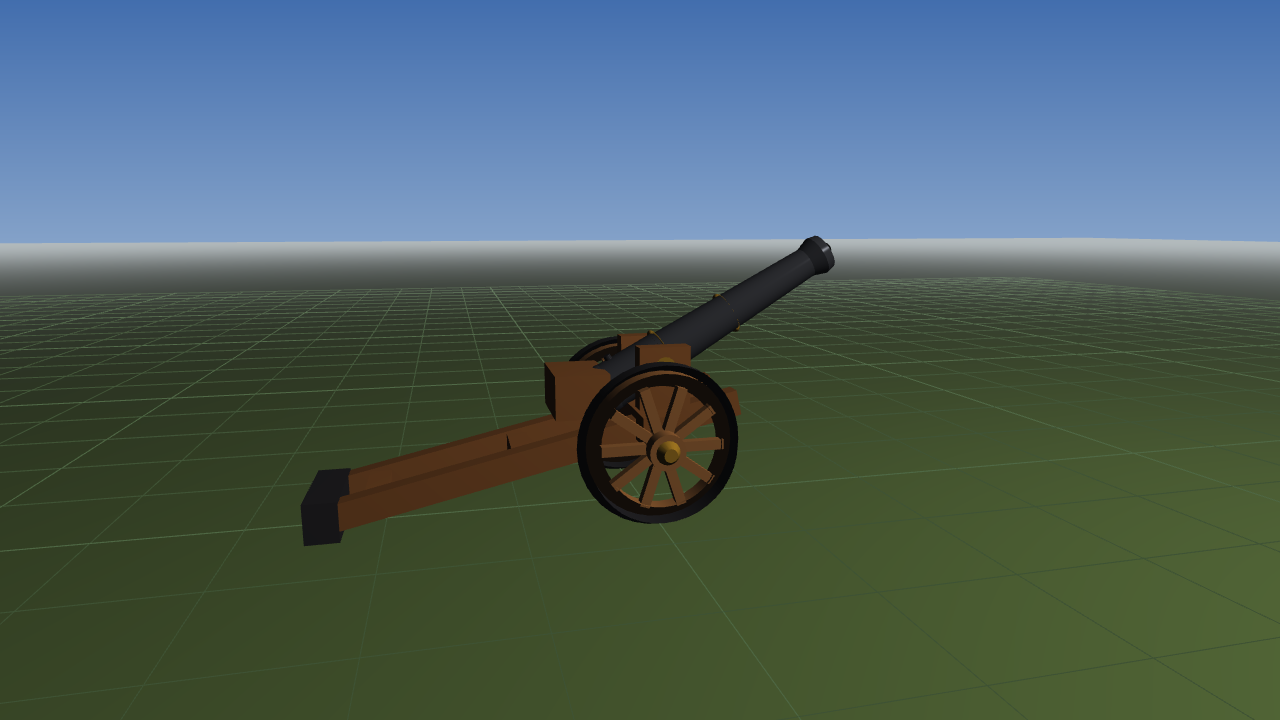
\includegraphics[width=\linewidth]{09_recoil_rest}\caption{at rest, $\rho=0$}
  \end{subfigure}\hfill
  \begin{subfigure}{0.49\linewidth}
    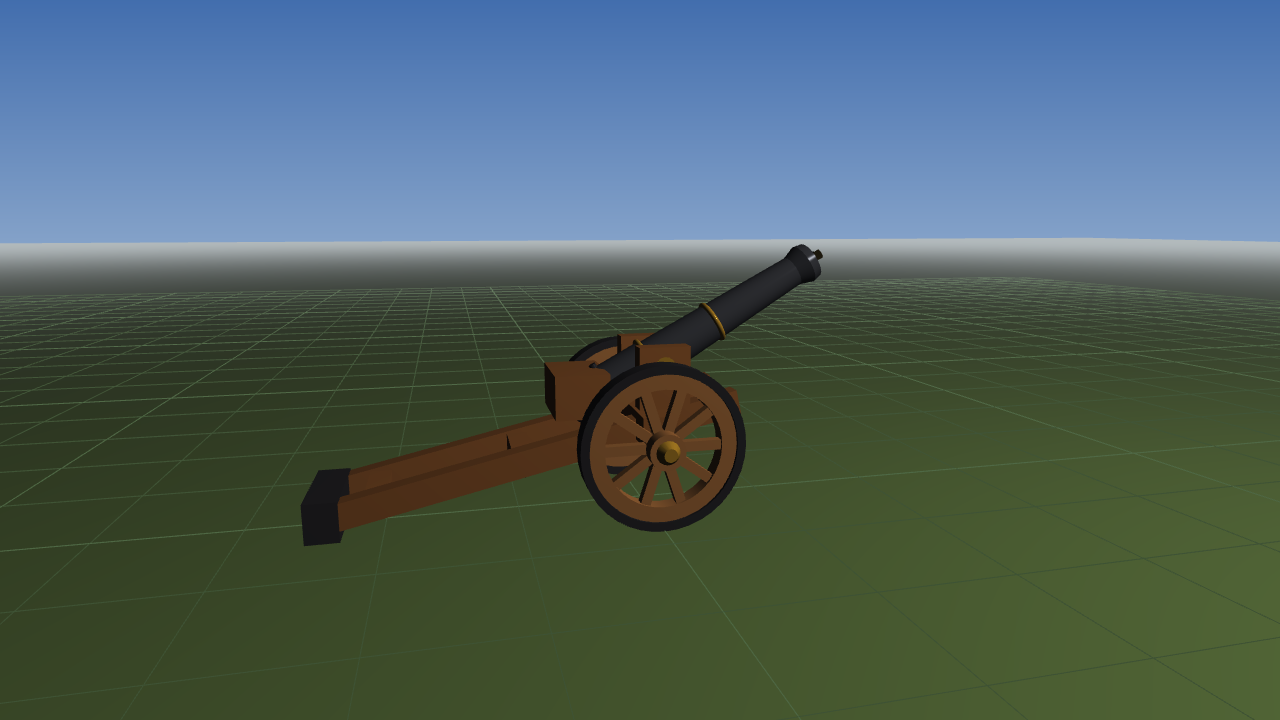
\includegraphics[width=\linewidth]{08_recoil}\caption{$t=0.11$\,s after firing, near $\rho_{\max}$}
  \end{subfigure}
  \caption{Recoil.  The barrel has slid back along its \emph{own} axis --- note
  that the breech has moved behind the cheeks while the trunnions and the whole
  carriage have not moved at all.}
  \label{fig:recoil}
\end{figure}

Because the translation $\bT(-\rho,0,0)$ sits \emph{inside} the elevation
rotation, the world-space displacement is automatically along the elevated
barrel:
$\Delta\bm{q}=-\rho(\cos\theta,\sin\theta,0)$.  At $\theta=25^\circ$ and
$\rho=0.30$\,m, \texttt{verify.py} measures $(-0.2719,-0.1268,0)$\,m against a
predicted $(-0.2719,-0.1268,0)$\,m.

\subsection{Projectile motion}

The ball leaves the muzzle at $\bm{q}$ (equation~\ref{eq:muzzle}) with velocity
$\bm{v}_0=v_m\bm{d}$, $v_m=15$\,m/s, and thereafter feels only
$\bm{g}=(0,-9.81,0)\;\mathrm{m/s^2}$:

\begin{equation}
\bm{p}(t)=\bm{q}+\bm{v}_0 t+\tfrac12\bm{g}t^2 .
\end{equation}

Solving the vertical component for the height $y_f$ at which the ball stops
gives the flight time and the range

\begin{equation}
t_f=\frac{v_m\sin\theta+\sqrt{(v_m\sin\theta)^2+2g\,(q_y-y_f)}}{g},
\qquad
X=v_m\cos\theta\; t_f .
\label{eq:range}
\end{equation}

The HUD displays \eqref{eq:range} live so the analytic prediction can be read
off while the simulated ball is still in the air.  The simulation itself uses the
same semi-implicit Euler scheme as the recoil.  For constant acceleration that
scheme has an exactly known bias: after $n$ steps of size $\Delta t$,

\begin{equation}
\bm{p}_n=\bm{q}+n\Delta t\,\bm{v}_0+\bm{g}\,\frac{n(n+1)}{2}\Delta t^2
       =\underbrace{\bm{q}+\bm{v}_0t+\tfrac12\bm{g}t^2}_{\text{exact}}
         +\tfrac12\bm{g}\,\Delta t\,t ,
\label{eq:eulerbias}
\end{equation}

i.e.\ the numerical ball sits $\tfrac12 g\Delta t\,t$ \emph{below} the true
parabola, so it lands slightly early and slightly short.  At $\Delta t=1/240$\,s
and $t\approx1.8$\,s that is about $3.7$\,cm, and indeed every simulated range
below is a little under the analytic one:

\begin{table}[H]
\centering\small
\begin{tabular}{@{}rrrrrr@{}}
\toprule
$\theta$ & $t_f$ exact (s) & $t_f$ sim (s) & $X$ exact (m) & $X$ sim (m) & rel.\ error \\
\midrule
$10^\circ$ & 0.8598 & 0.8583 & 12.7015 & 12.6794 & 0.174\,\% \\
$20^\circ$ & 1.3090 & 1.3083 & 18.4506 & 18.4415 & 0.050\,\% \\
$30^\circ$ & 1.7578 & 1.7542 & 22.8348 & 22.7873 & 0.208\,\% \\
$35^\circ$ & 1.9717 & 1.9708 & 24.2265 & 24.2162 & 0.043\,\% \\
$45^\circ$ & 2.3645 & 2.3625 & 25.0796 & 25.0581 & 0.086\,\% \\
\bottomrule
\end{tabular}
\caption{Simulated flight against the closed-form parabola, $\Delta t=1/240$\,s.
Note that the optimum elevation is not $45^\circ$ in general --- it is
$45^\circ$ only for a launch and landing at the same height; firing from
$q_y\approx2$\,m shifts the optimum a little below it.}
\end{table}

On contact the ball is reflected with restitution $e=0.35$ and tangential
damping $0.72$, $v_y\leftarrow -e\,v_y$, and is put to rest once
$|v_y|<0.8$\,m/s, which stops the infinite bouncing that a constant-restitution
model would otherwise produce.

\begin{figure}[H]
  \centering
  \begin{subfigure}{0.49\linewidth}
    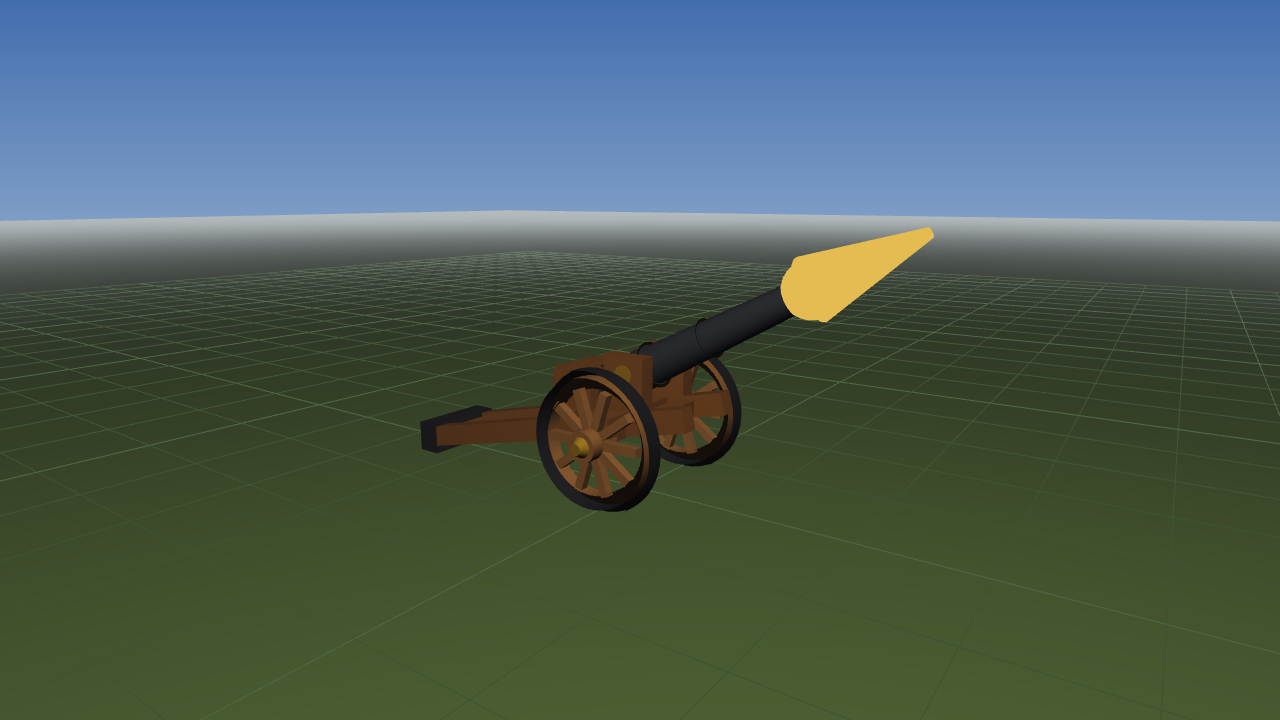
\includegraphics[width=\linewidth]{10_muzzle_flash}
    \caption{$t=14$\,ms: flash, ball leaving}
  \end{subfigure}\hfill
  \begin{subfigure}{0.49\linewidth}
    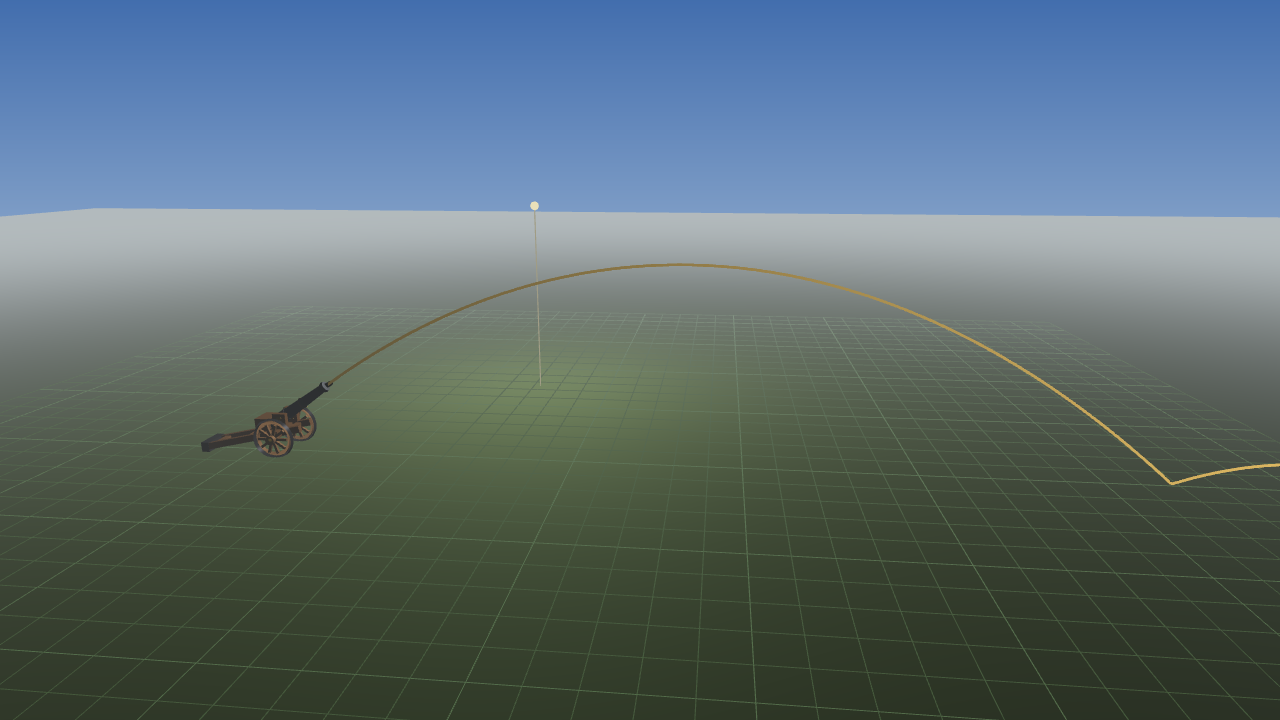
\includegraphics[width=\linewidth]{12_projectile_arc}
    \caption{the completed parabola, $\theta=35^\circ$}
  \end{subfigure}
  \caption{Firing.  The trail is a poly-line of the ball's own history, so the
  shape in (b) \emph{is} the integrated trajectory, not a drawn curve.  Its span
  matches the $24.2$\,m predicted by \eqref{eq:range}.}
  \label{fig:arc}
\end{figure}

\subsection{Viewing and projection}
\label{sec:view}

\paragraph{Camera.}  The camera orbits a target $\bm{t}$ (the cannon, optionally
offset down-range) at azimuth $\alpha$, elevation $\beta$ and distance $r$:

\begin{equation}
\bm{e}=\bm{t}+r\bigl(\cos\beta\cos\alpha,\;\sin\beta,\;\cos\beta\sin\alpha\bigr).
\end{equation}

\texttt{gluLookAt} then builds an orthonormal eye basis from $\bm{e}$, $\bm{t}$
and the up hint $\bm{u}_h=(0,1,0)$:

\begin{equation}
\bm{f}=\frac{\bm{t}-\bm{e}}{\|\bm{t}-\bm{e}\|},\qquad
\bm{s}=\frac{\bm{f}\times\bm{u}_h}{\|\bm{f}\times\bm{u}_h\|},\qquad
\bm{u}=\bm{s}\times\bm{f},
\end{equation}

\begin{equation}
\bm{V}=
\begin{pmatrix}
s_x&s_y&s_z&0\\ u_x&u_y&u_z&0\\ -f_x&-f_y&-f_z&0\\ 0&0&0&1
\end{pmatrix}
\bT(-\bm{e}).
\end{equation}

The rows are the eye basis because the matrix is the \emph{inverse} of the
camera's placement: $\bm{V}=(\bm{R}\bT(\bm{e}))^{-1}=\bT(-\bm{e})\bm{R}^{\mathsf T}$
written out.  The third row is negated because OpenGL's eye space looks down
$-Z$.  Pitch is clamped to $[-5^\circ,85^\circ]$ so $\bm{f}$ never becomes
parallel to $\bm{u}_h$, which would make $\bm{s}$ undefined.

\paragraph{Perspective.}  With a vertical field of view $\vartheta=50^\circ$,
aspect $a=w/h$, and near/far planes $n=0.1$, $f=200$,
$\texttt{gluPerspective}$ loads

\begin{equation}
\bm{P}=
\begin{pmatrix}
\frac{\cot(\vartheta/2)}{a}&0&0&0\\[2pt]
0&\cot(\vartheta/2)&0&0\\[2pt]
0&0&\frac{f+n}{n-f}&\frac{2fn}{n-f}\\[2pt]
0&0&-1&0
\end{pmatrix},
\qquad \cot(25^\circ)=2.1445 .
\end{equation}

The $-1$ in the last row copies $-z_{\text{eye}}$ into $w_{\text{clip}}$; the
subsequent perspective divide by $w$ is what makes distant objects small, and it
is also what makes depth non-linear:

\begin{equation}
z_{\text{ndc}}=\frac{f+n}{n-f}+\frac{2fn}{(n-f)\,(-z_{\text{eye}})}
\;\Longrightarrow\;
\text{half the depth buffer is spent inside } z_{\text{eye}}\in[-2n,-n].
\end{equation}

This is why $n=0.1$\,m and not $0.001$\,m: with the far plane at 200\,m, a near
plane a thousand times closer would crush the usable depth precision and produce
z-fighting on the barrel bands, which are only 2\,cm thick.

\begin{figure}[H]
  \centering
  \begin{subfigure}{0.32\linewidth}
    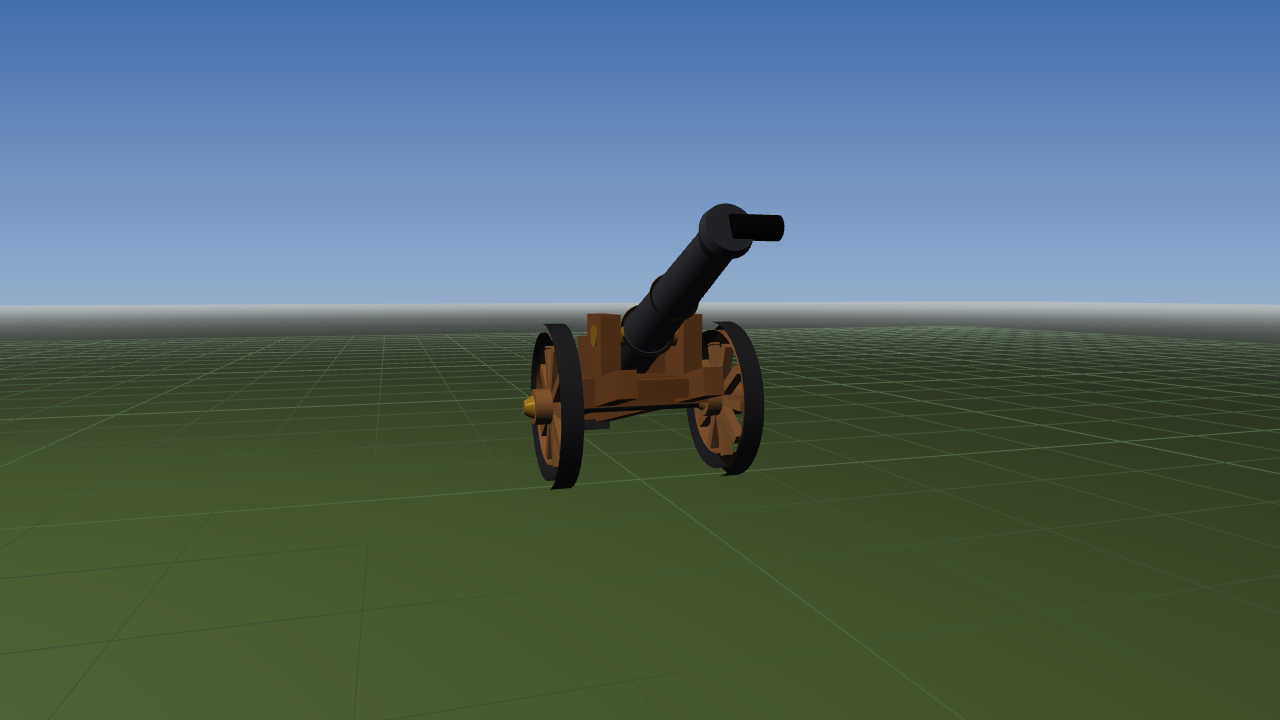
\includegraphics[width=\linewidth]{20_cam_low}\caption{low hero}
  \end{subfigure}\hfill
  \begin{subfigure}{0.32\linewidth}
    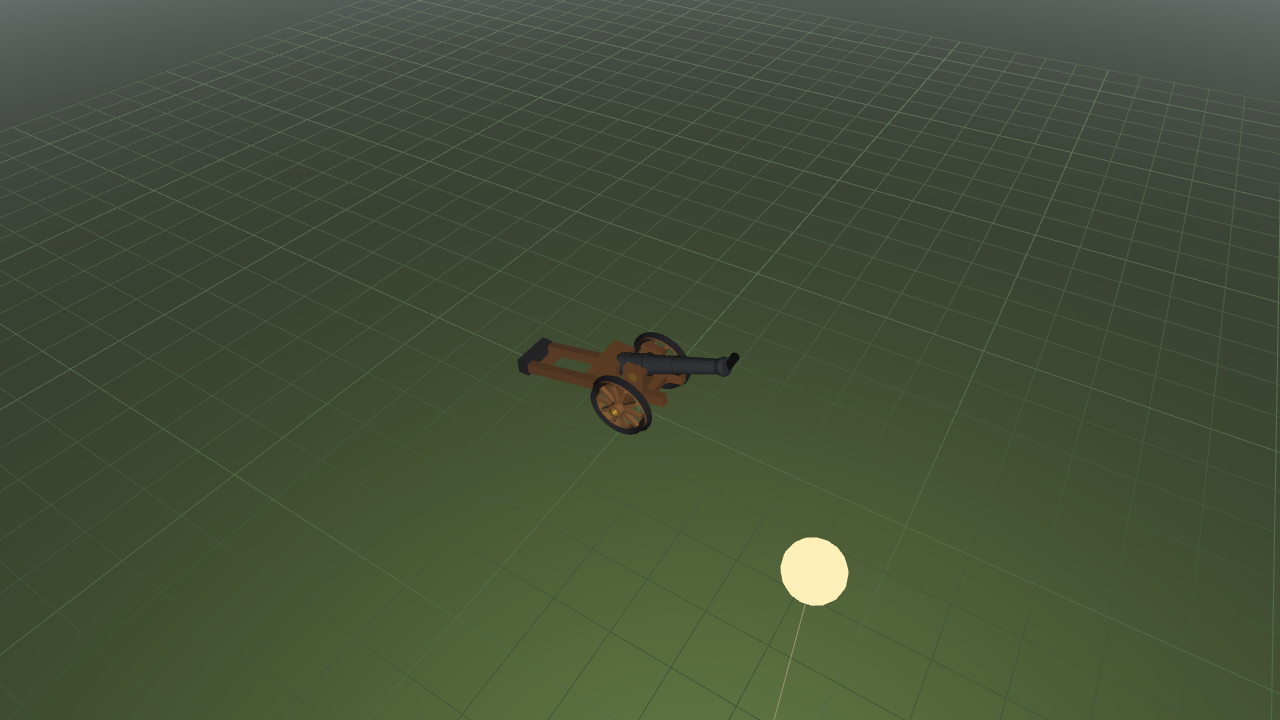
\includegraphics[width=\linewidth]{21_cam_overview}\caption{high overview}
  \end{subfigure}\hfill
  \begin{subfigure}{0.32\linewidth}
    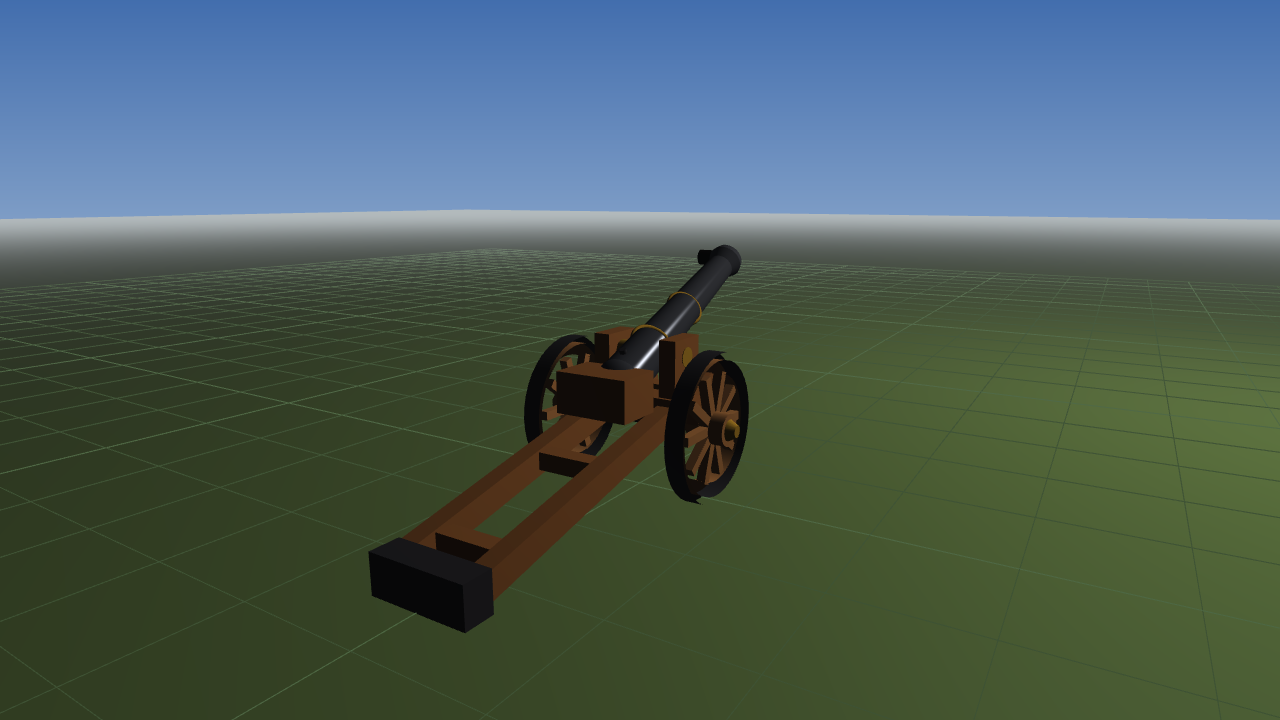
\includegraphics[width=\linewidth]{22_cam_downrange}\caption{down-range}
  \end{subfigure}
  \caption{Three of the five camera presets (\key{C}).  Perspective foreshortening
  is obvious in the grid: equal 1\,m squares converge towards the horizon.}
  \label{fig:cams}
\end{figure}

\subsection{Normals}

\paragraph{The normal matrix.}  A normal is not a direction that can be
transformed by $\bM$.  If $\bm{t}$ is a surface tangent, then
$\bN\cdot\bm{t}=0$ must still hold after transforming, i.e.\
$\bN'\cdot(\bm{M}\bm{t})=0$.  Substituting $\bN'=\bm{A}\bN$ gives
$\bN^{\mathsf T}\bm{A}^{\mathsf T}\bm{M}\bm{t}=0$ for all $\bm{t}$, so
$\bm{A}^{\mathsf T}\bm{M}=\bm{I}$ and

\begin{equation}
\bm{A}=(\bm{M}^{-1})^{\mathsf T},
\end{equation}

which is what \texttt{gl\_NormalMatrix} contains (the upper-left $3\times3$ of
the modelview, inverted and transposed).  This project uses only translations
and rotations, for which $(\bm{M}^{-1})^{\mathsf T}=\bm{M}$, so the distinction
is invisible here --- but it is the reason the shader is written with
\texttt{gl\_NormalMatrix} rather than \texttt{mat3(gl\_ModelViewMatrix)}, and it
would matter the moment a non-uniform \texttt{glScalef} were introduced.

\paragraph{Analytic normals for a truncated cone.}  Nearly every part of the
cannon --- barrel sections, muzzle swell, axle, hub, wheel rims --- is a
truncated cone, so its normal is worth deriving properly.  Parameterise the
lateral surface from radius $r_0$ at $z=0$ to $r_1$ at $z=h$:

\begin{equation}
\bP(\phi,t)=\bigl(r(t)\cos\phi,\;r(t)\sin\phi,\;h\,t\bigr),
\qquad r(t)=r_0+(r_1-r_0)t,\quad t\in[0,1].
\end{equation}

The two tangents are
$\partial\bP/\partial\phi=(-r\sin\phi,\;r\cos\phi,\;0)$ and
$\partial\bP/\partial t=\bigl((r_1-r_0)\cos\phi,\;(r_1-r_0)\sin\phi,\;h\bigr)$,
and their cross product is

\begin{equation}
\frac{\partial\bP}{\partial\phi}\times\frac{\partial\bP}{\partial t}
= r\bigl(h\cos\phi,\;h\sin\phi,\;r_0-r_1\bigr)
\;\;\Longrightarrow\;\;
\boxed{\;\bN=\frac{(h\cos\phi,\;h\sin\phi,\;r_0-r_1)}
                  {\sqrt{h^2+(r_1-r_0)^2}}\;}
\label{eq:conenormal}
\end{equation}

The radius factor $r$ divides out, so the normal depends only on $\phi$ --- it
is constant along each ruling, which is exactly why a cone shades with straight
highlight bands.  For a plain cylinder ($r_0=r_1$) it collapses to the familiar
$(\cos\phi,\sin\phi,0)$; the naive guess of using that for a \emph{tapered}
section is wrong by $\arctan\frac{r_0-r_1}{h}$, which for the barrel's chase is
$2.0^\circ$ --- small, but enough to misplace a tight specular highlight.
Check~5 of \texttt{verify.py} confirms \eqref{eq:conenormal} is unit length to
$2.2\times10^{-16}$ and orthogonal to both tangents to $1.8\times10^{-17}$.

Spheres use $\bN=\bP/r$, and the torus (the brass astragal rings) uses
$\bN=(\cos\alpha\cos\beta,\;\sin\alpha\cos\beta,\;\sin\beta)$ for tube angle
$\beta$ around ring angle $\alpha$.

\subsection{The Phong reflection model}
\label{sec:phong}

\begin{figure}[H]
\centering
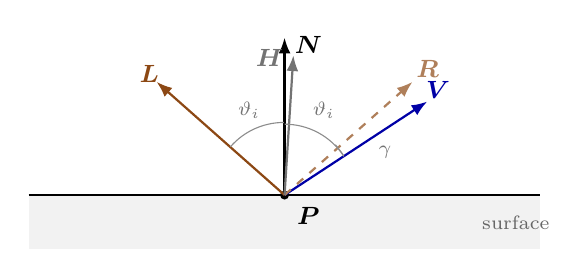
\begin{tikzpicture}[scale=1.25,every node/.style={font=\small}]
  \fill[black!5] (-2.6,-0.55) rectangle (2.6,0);
  \draw[line width=0.7pt] (-2.6,0) -- (2.6,0);
  \node[font=\scriptsize,black!60] at (2.35,-0.28) {surface};
  \coordinate (P) at (0,0);
  \fill (P) circle (1.3pt);
  \node[below right=1pt and 1pt of P] {$\bP$};
  \draw[-{Latex[length=2mm]},thick] (P) -- node[right,pos=0.95]{$\bN$} (0,1.6);
  \draw[-{Latex[length=2mm]},thick,accent] (P) -- node[above left,pos=0.9]{$\bL$} (-1.30,1.15);
  \draw[-{Latex[length=2mm]},thick,blue!65!black] (P) -- node[above right,pos=0.92]{$\bV$} (1.45,0.95);
  \draw[-{Latex[length=2mm]},thick,accent!70,dashed] (P) -- node[above right,pos=0.95]{$\bR$} (1.30,1.15);
  \draw[-{Latex[length=2mm]},thick,black!55] (P) -- node[left,pos=0.98]{$\bH$} (0.09,1.42);
  \draw[black!45] (-0.55,0.49) arc (139:90:0.72);
  \node[font=\scriptsize,black!55] at (-0.36,0.86) {$\vartheta_i$};
  \draw[black!45] (0,0.72) arc (90:33:0.72);
  \node[font=\scriptsize,black!55] at (0.40,0.86) {$\vartheta_i$};
  \draw[black!45] (0.60,0.40) arc (33:41:1.0);
  \node[font=\scriptsize,black!55] at (1.02,0.44) {$\gamma$};
\end{tikzpicture}
\caption{The vectors of the Phong model at a shading point.  $\bR$ is $\bL$
mirrored about $\bN$; the specular term falls off as $\cos^n\gamma$.  Blinn's
variant replaces $\gamma$ with the angle between $\bN$ and the half-vector
$\bH$.}
\label{fig:phongvec}
\end{figure}

Each fragment's colour is

\begin{equation}
\boxed{
\bm{I}= \bm{m}_e
     + \bm{k}_a\!\otimes\!\bm{i}_a^{\text{glob}}
     + \frac{1}{k_c+k_l d+k_q d^2}
       \Bigl[\bm{k}_a\!\otimes\!\bm{i}_a
           + \bm{k}_d\!\otimes\!\bm{i}_d\max(\bN\!\cdot\!\bL,0)
           + \bm{k}_s\!\otimes\!\bm{i}_s\max(\bR\!\cdot\!\bV,0)^{\,n}\Bigr]}
\label{eq:phong}
\end{equation}

where $\otimes$ is component-wise multiplication over the RGB channels,
$d=\|\bP_{\text{light}}-\bP\|$, and

\begin{equation}
\bL=\frac{\bP_{\text{light}}-\bP}{d},\qquad
\bV=\frac{-\bP}{\|\bP\|}\ \text{(eye space)},\qquad
\bR=2(\bN\cdot\bL)\bN-\bL .
\end{equation}

The three terms do three different jobs, and the project can show each in
isolation:

\begin{description}[itemsep=2pt,topsep=3pt,leftmargin=16mm,style=nextline]
  \item[Ambient] a constant floor standing in for all the light that has bounced
    off everything else.  Pressing \key{L} kills the direct light and leaves
    only $\bm{m}_e+\bm{k}_a\otimes\bm{i}_a^{\text{glob}}$ ---
    Figure~\ref{fig:lightoff}(c).  The scene becomes a flat silhouette, which is
    the point: ambient alone carries no shape information.
  \item[Diffuse] Lambert's cosine law, $\bN\cdot\bL$: it depends on where the
    light is but not on where the eye is, so it does not move when you orbit.
    This is what gives the carriage its solidity.
  \item[Specular] the mirror lobe, $(\bR\cdot\bV)^n$: it depends on the eye, so
    it slides across the barrel as either the camera or the light moves
    (Figure~\ref{fig:lightmove}).  The exponent $n$ controls tightness ---
    $n=8$ for wood spreads a weak sheen over the whole plank, $n=96$ for iron
    concentrates it into the thin streak seen in Figure~\ref{fig:materials}.
\end{description}

\paragraph{Attenuation and the light type.}  With $w=1$ the light is a point
source at a finite distance, $\bL$ is recomputed per fragment, and the
$1/(k_c+k_ld+k_qd^2)$ factor applies ($k_c=1$, $k_l=0.010$, $k_q=0.0004$).
Pressing \key{N} sets $w=0$: the position becomes a direction, $\bL$ is constant
everywhere, and attenuation is disabled --- the sun-at-infinity model.  The
difference is easiest to see on the large ground plane, which loses its pool of
light and becomes uniformly lit.

\paragraph{Materials.}  Two of these are required to contrast; the project ships
five.

\begin{table}[H]
\centering\small
\begin{tabular}{@{}lcccc@{}}
\toprule
\textbf{Material} & $\bm{k}_a$ & $\bm{k}_d$ & $\bm{k}_s$ & $n$ \\
\midrule
Oak (carriage)      & (0.14,\,0.09,\,0.05) & (0.52,\,0.32,\,0.16) & (0.10,\,0.08,\,0.06) & 8 \\
Light oak (wheels)  & (0.16,\,0.11,\,0.06) & (0.60,\,0.40,\,0.22) & (0.12,\,0.10,\,0.08) & 10 \\
Cast iron (barrel)  & (0.06,\,0.07,\,0.08) & (0.19,\,0.20,\,0.23) & (0.92,\,0.94,\,1.00) & 96 \\
Brass (fittings)    & (0.16,\,0.12,\,0.04) & (0.62,\,0.47,\,0.13) & (0.85,\,0.75,\,0.45) & 64 \\
Iron tyre           & (0.05,\,0.05,\,0.06) & (0.13,\,0.13,\,0.15) & (0.55,\,0.55,\,0.60) & 48 \\
Field (ground)      & (0.10,\,0.13,\,0.08) & (0.34,\,0.44,\,0.24) & (0.04,\,0.05,\,0.04) & 4 \\
\bottomrule
\end{tabular}
\caption{Phong coefficients.  Wood and iron differ by roughly $9\times$ in
specular strength and $12\times$ in exponent --- that ratio, not the base colour,
is what makes one look like timber and the other like metal.}
\label{tab:materials}
\end{table}

\begin{figure}[H]
  \centering
  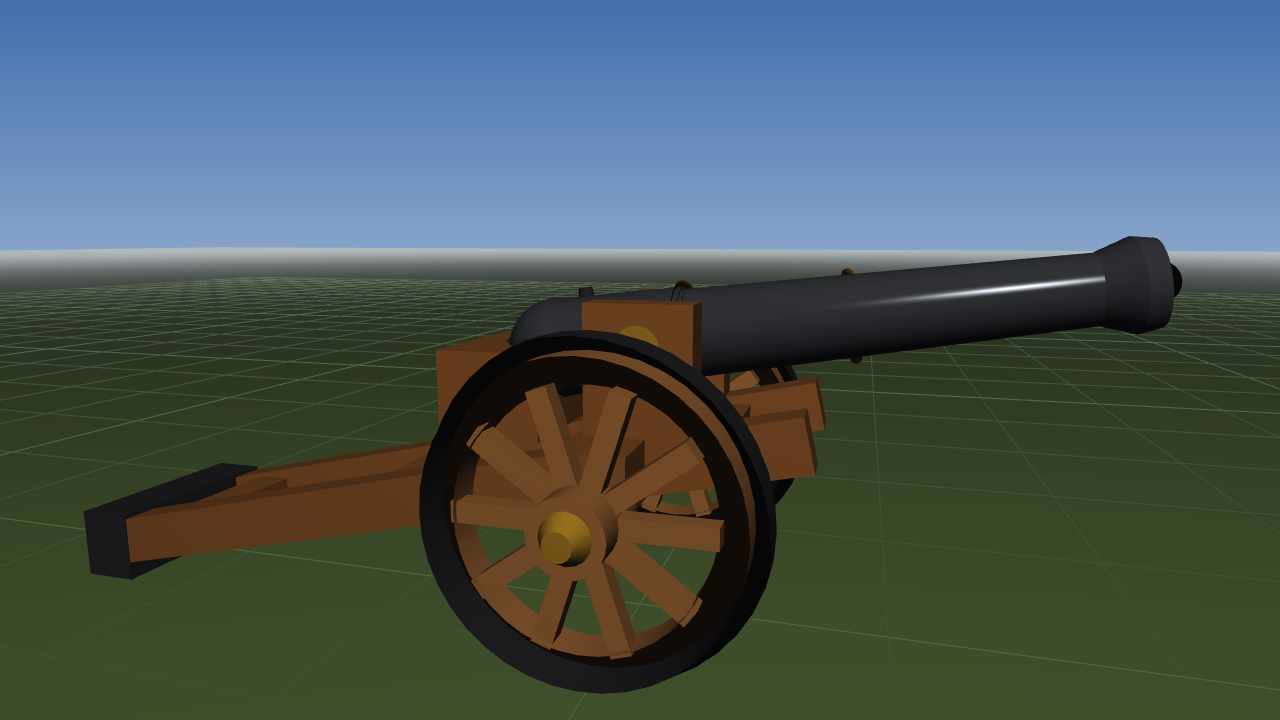
\includegraphics[width=0.86\linewidth]{18_materials}
  \caption{Two materials under one light.  The oak beams and spokes show a broad,
  almost invisible sheen ($k_s\approx0.1$, $n=8$) and read as matte; the barrel
  carries a narrow white streak ($k_s\approx0.95$, $n=96$) and reads as polished
  iron.  The brass hub cap sits between the two.  Nothing here is a painted
  highlight --- all of it comes out of \eqref{eq:phong}.}
  \label{fig:materials}
\end{figure}

\paragraph{Why the highlight needs the light in the right place.}  A specular
streak appears where the mirror condition $\bR=\bV$ is met, equivalently where
$\bL+\bV\parallel\bN$.  On a cylinder of axis $\hat{\bm{a}}$ every normal
satisfies $\bN\cdot\hat{\bm{a}}=0$, so a \emph{perfect} highlight exists only if

\begin{equation}
(\bL+\bV)\cdot\hat{\bm{a}}=0 ,
\label{eq:cylhighlight}
\end{equation}

that is, only if the light and the eye lie on opposite sides of the plane
through the barrel perpendicular to its axis.  When they lie on the same side,
$\max_\phi(\bN\cdot\bH)$ can be as low as $0.89$, and raised to $n=96$ that is
$1.4\times10^{-5}$ --- effectively black.  This is not a defect; it is
\eqref{eq:phong} behaving correctly, and it is why the light is placed at
azimuth $122^\circ$ against a camera at $58^\circ$ for
Figure~\ref{fig:shading}.

\begin{figure}[H]
  \centering
  \begin{subfigure}{0.32\linewidth}
    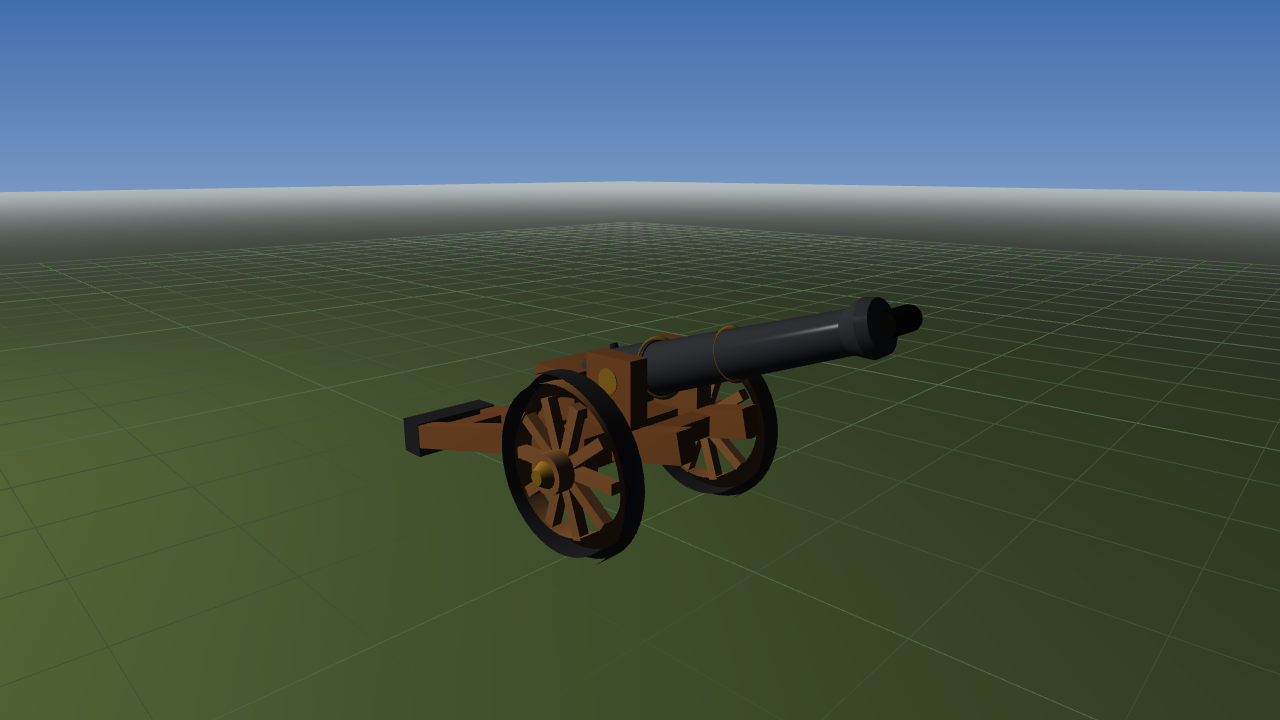
\includegraphics[width=\linewidth]{16_light_left}\caption{light at $120^\circ$}
  \end{subfigure}\hfill
  \begin{subfigure}{0.32\linewidth}
    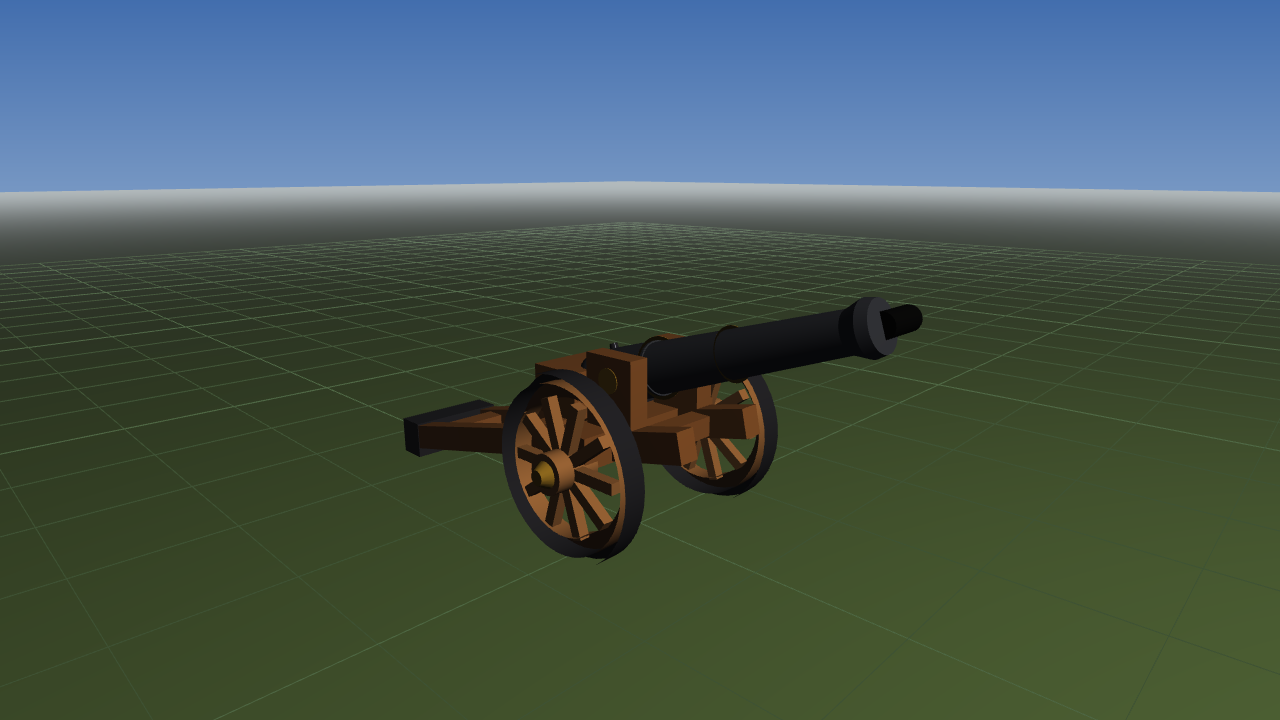
\includegraphics[width=\linewidth]{17_light_right}\caption{light at $10^\circ$}
  \end{subfigure}\hfill
  \begin{subfigure}{0.32\linewidth}
    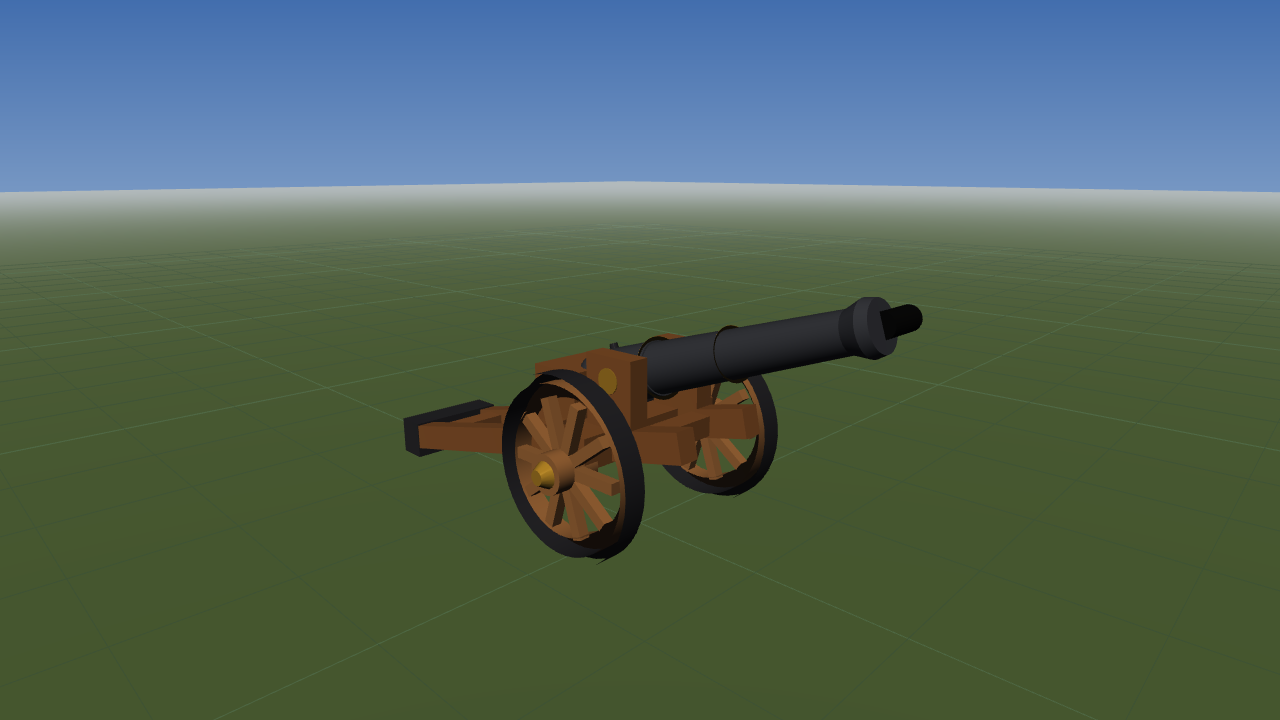
\includegraphics[width=\linewidth]{19_light_directional}\caption{directional ($w=0$)}
  \end{subfigure}
  \caption{Identical camera, identical materials, moved light.  In (a)
  condition~\eqref{eq:cylhighlight} is satisfied and the barrel carries a bright
  streak; in (b) the light has swung to the eye's own side and the streak
  vanishes while the diffuse shading merely shifts.  In (c) the same light is
  made directional: the falloff across the ground disappears.}
  \label{fig:lightmove}
\end{figure}

\subsection{Gouraud versus Phong shading}

The reflection model of \S\ref{sec:phong} says \emph{what} to compute; shading
says \emph{where}.  The fixed-function pipeline evaluates \eqref{eq:phong} once
per vertex and interpolates the resulting colour across the triangle (Gouraud
shading).  The GLSL path interpolates the \emph{normal} and evaluates
\eqref{eq:phong} once per fragment (Phong shading).  Since a specular lobe of
exponent 96 is far narrower than a triangle, per-vertex evaluation either misses
the highlight entirely or smears it into a polygonal blob.

Pressing \key{F} switches paths at runtime.  Crucially, both paths read the
\emph{same} \texttt{glMaterial}/\texttt{glLight} state --- the shader uses the
legacy \texttt{gl\_FrontMaterial} and \texttt{gl\_LightSource[0]} built-ins --- so
the comparison isolates the shading frequency and nothing else.

\begin{figure}[H]
  \centering
  \begin{subfigure}{0.49\linewidth}
    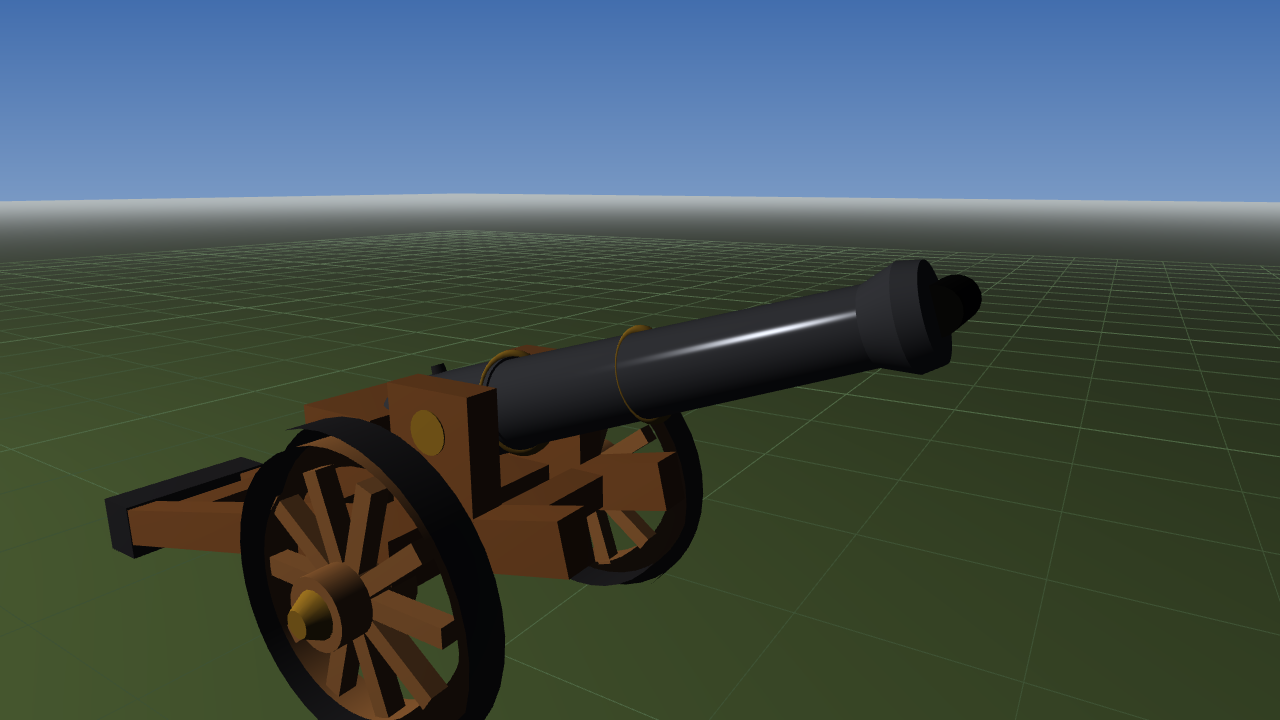
\includegraphics[width=\linewidth]{13_shading_phong}
    \caption{per-fragment Phong}
  \end{subfigure}\hfill
  \begin{subfigure}{0.49\linewidth}
    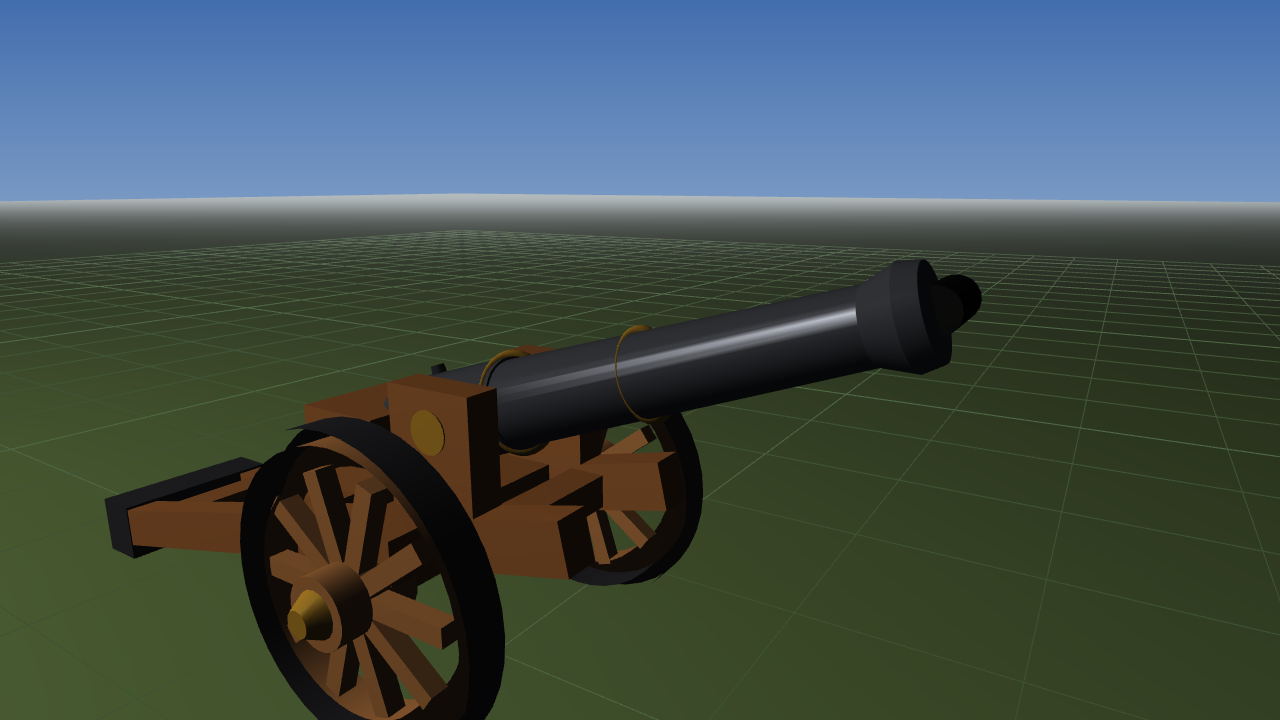
\includegraphics[width=\linewidth]{14_shading_gouraud}
    \caption{per-vertex Gouraud}
  \end{subfigure}\\[2mm]
  \begin{subfigure}{0.49\linewidth}
    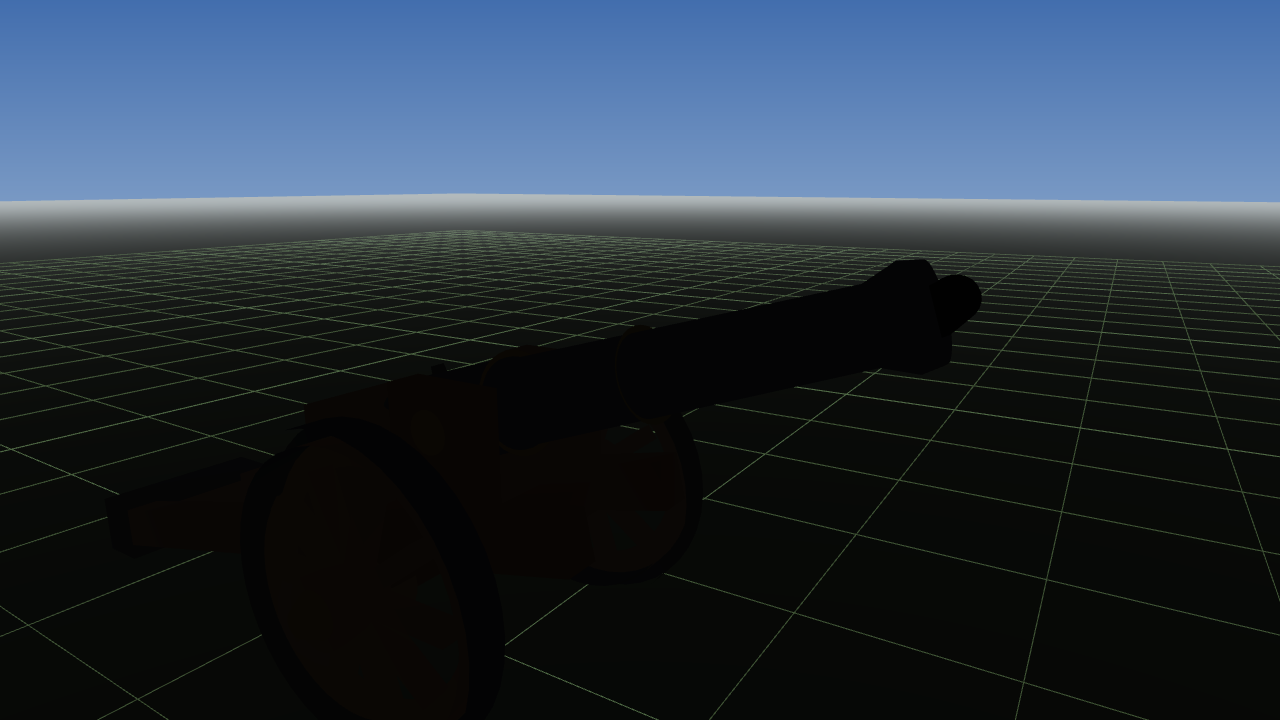
\includegraphics[width=\linewidth]{15_light_off}
    \caption{light off: the ambient term alone}
  \end{subfigure}
  \caption{The same frame under the two shading paths, and with the direct light
  disabled.  Measured over the whole frame, (a) and (b) differ by more than
  $4/255$ on $8.82\,\%$ of pixels, with a maximum channel difference of
  $88/255$; peak luminance is $255$ under Phong against $205$ under Gouraud, and
  the Gouraud highlight is visibly banded along the 40 slices of the tube.}
  \label{fig:shading}
  \label{fig:lightoff}
\end{figure}

\subsection{Atmospheric fog}

The ground plane is finite ($100\times100$\,m), and its edge would otherwise be
a hard line across the sky.  Both paths therefore apply exponential-squared fog
in eye space,

\begin{equation}
f=e^{-(\varrho z_{\text{eye}})^2},\qquad
\bm{C}=f\,\bm{C}_{\text{lit}}+(1-f)\,\bm{C}_{\text{fog}},\qquad
\varrho = 0.020\ \mathrm{m^{-1}},
\end{equation}

and the lowest stop of the sky gradient is set to $\bm{C}_{\text{fog}}$, so the
plane dissolves into the horizon.  At the 3--9\,m working distance of the cannon
$f>0.99$, so the model itself is essentially unfogged.

%=============================================================================
\section{Implementation notes}
%=============================================================================

\subsection{The shader}

\begin{lstlisting}[language=GLSL,caption={The fragment shader --- equation~\eqref{eq:phong}, verbatim.},captionpos=b]
varying vec3 vNormalEye;   // interpolated normal  -> Phong (not Gouraud) shading
varying vec3 vPosEye;
uniform bool uLightEnabled, uBlinn;
uniform vec3 uFogColor;  uniform float uFogDensity;

void main() {
    vec3 N = normalize(vNormalEye);
    vec3 color = gl_FrontLightModelProduct.sceneColor.rgb;   // emission + k_a * global ambient

    if (uLightEnabled) {
        vec4  lpos = gl_LightSource[0].position;   // already in eye space
        vec3  Lv   = lpos.xyz - vPosEye * lpos.w;  // w = 0  ->  directional
        float d    = length(Lv);
        vec3  L    = Lv / max(d, 1e-6);

        float att = 1.0;
        if (lpos.w > 0.5)
            att = 1.0 / (gl_LightSource[0].constantAttenuation
                       + gl_LightSource[0].linearAttenuation    * d
                       + gl_LightSource[0].quadraticAttenuation * d * d);

        vec3  V   = normalize(-vPosEye);           // local viewer
        float ndl = max(dot(N, L), 0.0);
        float spec = 0.0;
        if (ndl > 0.0) {
            if (uBlinn) { vec3 H = normalize(L + V);
                          spec = pow(max(dot(N, H), 0.0), gl_FrontMaterial.shininess); }
            else        { vec3 R = reflect(-L, N);
                          spec = pow(max(dot(R, V), 0.0), gl_FrontMaterial.shininess); }
        }
        color += att * (gl_LightSource[0].ambient.rgb  * gl_FrontMaterial.ambient.rgb
                      + gl_LightSource[0].diffuse.rgb  * gl_FrontMaterial.diffuse.rgb  * ndl
                      + gl_LightSource[0].specular.rgb * gl_FrontMaterial.specular.rgb * spec);
    }
    float z = length(vPosEye);
    color = mix(uFogColor, color, clamp(exp(-(uFogDensity*z)*(uFogDensity*z)), 0.0, 1.0));
    gl_FragColor = vec4(color, gl_FrontMaterial.diffuse.a);
}
\end{lstlisting}

If \texttt{glCompileShader} or \texttt{glLinkProgram} fails on any driver, the
exception is caught, \texttt{PhongShader.available} stays \texttt{False}, and the
program runs entirely on the fixed-function pipeline.  Nothing else in the code
has to know which path is live.

\paragraph{Blinn--Phong.}  Pressing \key{B} swaps $(\bR\cdot\bV)^n$ for
$(\bN\cdot\bH)^n$ with $\bH=\widehat{\bL+\bV}$.  Since the angle between $\bN$
and $\bH$ is about half the angle between $\bR$ and $\bV$, the Blinn lobe is
roughly twice as wide for the same $n$; matching the two requires
$n_{\text{Blinn}}\approx4n_{\text{Phong}}$.

\subsection{Drawing unlit geometry inside a lit frame}

The projectile trails, the light marker and the HUD are flat-coloured.  Simply
calling \texttt{glDisable(GL\_LIGHTING)} is not enough when a shader is bound,
because the shader ignores that state entirely and would keep shading them with
the last material --- an early version of this project drew the trails almost
black for exactly that reason.  \texttt{lighting.unlit} is a context manager that
drops out of both the shader and fixed-function lighting and restores whichever
was active:

\begin{lstlisting}[language=Python]
with unlit():                 # leaves the program, disables GL_LIGHTING
    glBegin(GL_LINE_STRIP)
    ...                       # glColor3f now actually reaches the framebuffer
    glEnd()
\end{lstlisting}

\subsection{Geometry budget}

\begin{table}[H]
\centering\small
\begin{tabular}{@{}lll@{}}
\toprule
\textbf{Part} & \textbf{Primitive} & \textbf{Tessellation} \\
\midrule
Trail beams, transoms, cheeks, spokes & box & 6 quads each \\
Barrel (breech, reinforce, chase, swell, bore) & truncated cones + sphere & 40 slices \\
Wheel tyre and felloe & tube (annulus) & 40 slices \\
Wheel hub, axle, trunnions & cylinders & 16--24 slices \\
Astragal rings & torus & $32\times12$ \\
Cannonball & UV sphere & $20\times14$ \\
Ground & tessellated quad grid & $150\times150$ \\
\bottomrule
\end{tabular}
\caption{The ground is finely tessellated on purpose: under the fixed-function
per-vertex path a single large quad would sample the point light at only four
corners and the pool of light would vanish.}
\end{table}

%=============================================================================
\section{Results}
%=============================================================================

The scene runs at the display refresh rate on the test machine; the HUD in
Figure~\ref{fig:hud} reports a measured frame rate obtained by timing 30
consecutive \texttt{render()} calls with \texttt{glFinish} barriers, not an
estimate.

\begin{figure}[H]
  \centering
  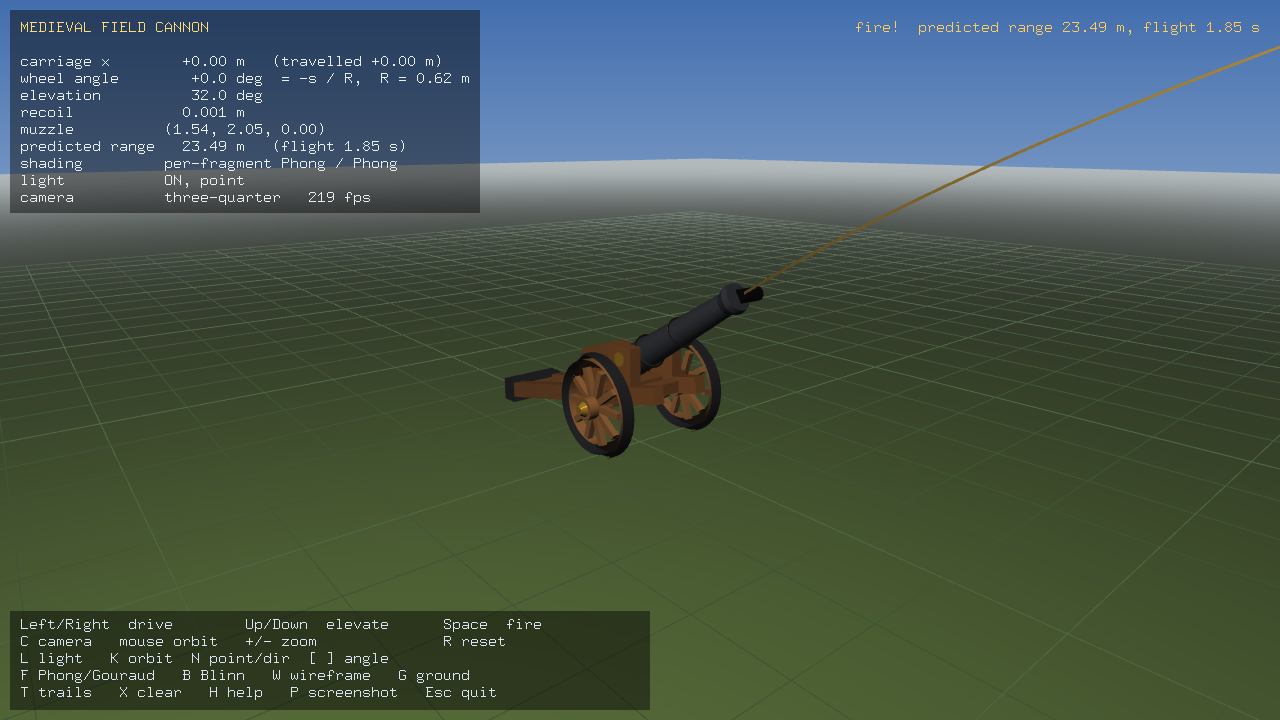
\includegraphics[width=\linewidth]{23_hud}
  \caption{The live HUD.  It reports the carriage position and distance
  travelled, the wheel angle beside the $-s/R$ rule that produced it, the
  elevation, the instantaneous recoil, the muzzle point from \eqref{eq:muzzle},
  and the analytic range prediction \eqref{eq:range} for the shot currently in
  the air.}
  \label{fig:hud}
\end{figure}

\begin{figure}[H]
  \centering
  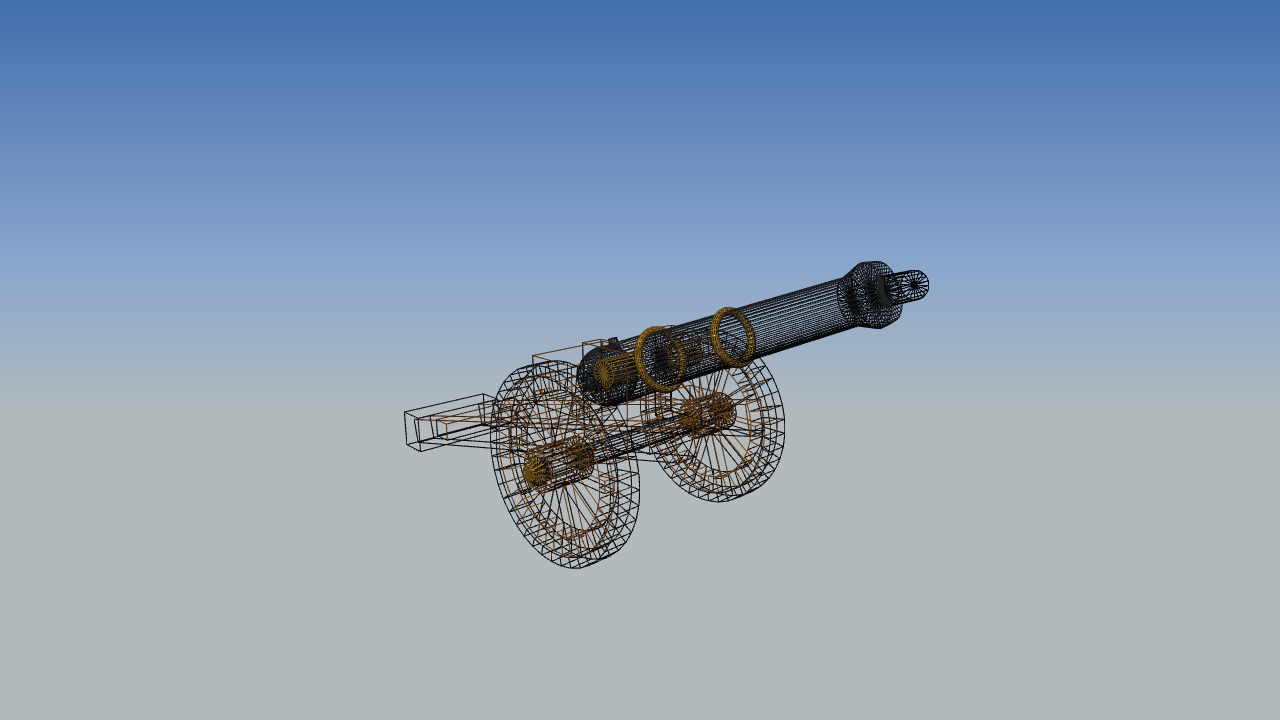
\includegraphics[width=0.8\linewidth]{02_wireframe}
  \caption{Wireframe (\key{W}).  The structure is visible: 10 box spokes per
  wheel, the annular tyre and felloe, the stack of truncated cones that forms
  the barrel, and the sphere at the breech.  No external model files are used ---
  every vertex is generated by \texttt{utils.py}.}
  \label{fig:wire}
\end{figure}

%=============================================================================
\section{Limitations and possible extensions}
%=============================================================================

\begin{itemize}[itemsep=2pt,topsep=3pt]
  \item \textbf{No shadows.}  The cannon does not cast one, which is the most
        noticeable absence.  A planar projection shadow onto $y=0$ would be a
        single extra matrix and would cost almost nothing.
  \item \textbf{One light.}  The rig supports \texttt{GL\_MAX\_LIGHTS}$=8$; the
        shader hard-codes \texttt{gl\_LightSource[0]} and would need a loop.
  \item \textbf{Legacy GLSL.}  Using the deprecated built-ins keeps the shader
        and fixed-function paths in perfect agreement --- ideal for the
        comparison in Figure~\ref{fig:shading} --- but a modern core-profile
        port would have to pass materials and lights as explicit uniforms.
  \item \textbf{Flat ground, no drag.}  The projectile ignores air resistance and
        the terrain is a plane; both are deliberate, per the brief's instruction
        to keep the scope tight.
  \item \textbf{No textures.}  All surface variety comes from the material
        coefficients in Table~\ref{tab:materials}, which is what makes the
        lighting model so legible in the figures.
\end{itemize}

%=============================================================================
\appendix
\section{Verification output}
\label{app:verify}
%=============================================================================

Produced by \texttt{python verify.py}; every number quoted in
\S4 comes from this run.

\lstinputlisting[basicstyle=\ttfamily\tiny,frame=single,
                 rulecolor=\color{black!25},backgroundcolor=\color{codebg}]{verification.txt}

\end{document}
